% Define document class
\documentclass[12pt]{report}
\usepackage{aas_macros}

% Citations
\usepackage{natbib}
\bibliographystyle{abbrvnat}
\setcitestyle{authoryear}

% Language 
\usepackage[utf8x]{inputenc}

% Layout and margins 
\usepackage[margin=1in]{geometry}
\usepackage{layout}
\usepackage{lastpage}
\usepackage{titling}

% Figures & tables 
\usepackage{graphicx,xcolor}
\usepackage{caption}
\usepackage{subcaption}
\usepackage{booktabs} % much better looking tables

% Math 
\usepackage{amsmath,amssymb,bm}
\DeclareMathOperator*{\argmax}{arg\,max}
\usepackage{siunitx} % for proper units 
\usepackage{esint} % various fancy integral symbols
\usepackage[bbgreekl]{mathbbol}

% Other packages
\usepackage{url}
\usepackage{epstopdf}
\usepackage[font=scriptsize]{caption} % smaller font for fig captions
\usepackage[section]{placeins}
%\usepackage{import}
% of references  

% Settings
\hfuzz=6pt % tolerance on hbox overflows

% Custom command
\newcommand{\ud}{\,\mathrm{d}}
\renewcommand{\vec}[1]{\boldsymbol{\mathbf{#1}}}

\hypersetup{
    colorlinks=true,
    allcolors=cyan,
}

% Begin!
\begin{document}

% Title
\title{\vspace{-15pt}\begin{center}
\includegraphics[width=0.4\linewidth]{static/misc/logo.jpg}\end{center}
    \vspace{20pt}
    \begin{center}
        School of Physics \& Astronomy
    \end{center}
    \vspace{20pt}
    \begin{center}
        \LARGE\textbf{Probabilistic modeling of astrophysical time series:
            gravitational microlensing and occultation mapping of planets and moons}
    \end{center}
    \vspace{20pt}
    \begin{center}
        Supervisor: Dr. Martin Dominik
    \end{center}
}

\maketitle
\tableofcontents

% Abstract 
\chapter*{Abstract}

Scientific progress in modern astronomy research commonly relies on gathering
large quantities of data using exceedingly precise instruments. The process
which ``generates'' these data consists of the physical phenomenon of interest
-- for instance, an exoplanet blocking or twisting the light of a distant star,
and the noise introduced by the measurement process and the presence of an
atmosphere The task for an astronomer is to first construct a \emph{model}
which describes the entire process which generated the data and to then ``fit''
that model to data. All models only approximate reality and the researcher has
to make a series of decisions during the model building process, everything
from how to process the raw data to which results to put in the abstract of a
paper. Advancements in computational statistics and machine learning in the
past decade or so have made it possible to fit ever more complex models to
data. These models are generally expressed in computer code which may contain
complex numerical algorithms, such as iterative solvers and numerical
integrals. In this thesis, I mostly focused on developing methods which enable
\emph{statistical inference} with these kinds of complex models in two
particular domains within astronomy, gravitational microlensing and occultation
mapping. The common theme between these two topics is that both deal with
accurately measuring the brightness of distant stars as a function of time with
the goal of inferring properties of exoplanets and stars. Broadly speaking, I
believe the biggest contribution of this thesis is providing a new lens for
looking at a particular set of old problems, a lens which incorporates recent
advancements from statistics, machine learning and computer science. More
specifically, I have developed a an open-source software package
\textsf{caustics}\footnote{\url{https://github.com/fbartolic/caustics}} which
enables fast and accurate computation of binary lens and triple lens
microlensing light curves and simultaneously provides exact \emph{gradients} of
the code outputs with respect to all its inputs. This is significant because it
for the first time enables the use of modern gradient based statistical
inference algorithms such as Hamiltonian Monte Carlo with microlensing light
curves. Microlensing is one of the major goals for the upcoming \emph{NASA
    Roman} telescope and the existing modeling methods are completely inadequate
for dealing with the scale of data which will come from \emph{Roman}. I also
propose a framework for dealing with issues which have plagued the field for
decades -- various pathologies in microlensing models and questions about the
interpretation of statistical results. Besides microlensing, I have also delved
into the field of occultation mapping of Solar System objects and exoplanets.
Together with collaborators, I have developed a novel statistical method for
reconstructing spatial maps of volcanic emission on Jupiter's moon Io using
infra-red occultation light curves. I applied the same method to exoplanets to
explore the exciting possibility of detecting weather changes on Hot Jupiters
by reconstructing two dimensional maps of the emission surface from simulated
\emph{JWST} secondary eclipse light curves. I found that planetary scale
changes in the emission pattern should be detectable with \emph{JWST}.

\newpage
\thispagestyle{empty}

% CHAPTER 1: Introduction
\chapter{Introduction}
\section{Context}

The key idea of the scientific revolution in the 16th century was to carefully
observe the world, build \emph{models} which describe some aspect of the
observed phenomenon, and finally and most importantly -- test those models to
see if they provide an accurate description of reality. Since the time of
Galileo, this process gave rise to the modern world and revolutionised our
understanding of the universe. Today we have amazingly accurate models of the
universe. Einstein's theory of \emph{General Relativity} which describes the
universe at a large scale and the \emph{Standard Model} which describes the
universe at the atomic and subatomic scales, both of which were developed in
the 20th century. In my opinion, the two most important questions for the
physical sciences in the 21st century and beyond are the following:
\begin{itemize}
    \item How do we combine the Standard Model and General Relativity to get a complete
          physical theory of the Universe?
    \item What is the origin and distribution of complex life in the Universe?
\end{itemize}

It used to be the case that conducting experiments with the potential to to
change our understanding of fundamental physics was relatively straightforward
and could be conducted by a single person or a small group of researchers. I
have in mind, for instance, Kepler's observations of planetary orbits, Ernest
Rutherford's experiments with atoms or Arthur Eddington's observations of the
Solar eclipse with the goal of testing General Relativity. The data gathering
process consisted of writing notes in a physical notebook and the analysis
hardly required complex statistics. Today the situation is more complicated
because much of the ``low-hanging fruit'' of scientific discovery (in the
physical sciences) has been exhausted and the use of computers is absolutely
central to the process. Progress today usually (but not always) requires
coordination between many scientists, engineers and software engineers building
highly complex experiments. Consider this list of some of the most notable
scientific discoveries in the past few decades:
\begin{itemize}
    \item  Discovery of accelerated expansion of the Universe
    \item  First sequencing of the human genome
    \item  Detection of the Higgs Boson
    \item  Paleogenomics studies of the origin of Homo Sapiens
    \item  Detection of gravitational waves by LIGO
    \item  Reconstruction of the first image of a Black Hole
\end{itemize}
All of these discoveries required gathering substantial amounts of data and the use of
relatively complex statistical analysis techniques.
Computation and statistical analysis are now absolutely central the process of scientific
discovery.

Simultaneously, in the past decade there's been a complete revolution in the
field of machine learning/AI thanks to the advent of deep learning and neural
networks. Besides the incredible progress on predicting patterns in language
and vision, deep learning has also been used in science for things like solving
the protein folding problem \citep{2021Natur.596..583J} and in mathematics for
the purpose of discovering novel conjectures and theorems
\citet{2021Natur.600...70D}. Deep learning has been less useful in physics and
astronomy so far but as I will argue in this thesis, some of the technologies
which underlie deep learning such as automatic differentiation and GPU
computing are going to be (if they aren't already) crucial for processing and
understanding complex datasets in physics and astronomy.

\begin{figure}
    \begin{centering}
        \includegraphics[width=0.8\linewidth]{figures/ads_keyword_bayesian.pdf}
        \caption{Number of NASA/ADS entries containing the keyword ``Bayesian'' per year.}
        \label{fig:ads_keyword_bayesian}
    \end{centering}
\end{figure}

There is another revolution worth mentioning. It is slightly less obvious than
the one in machine learning but nevertheless significant. In the past two
decades there has been a substantial increase in popularity of Bayesian
statistics. Fig~\ref{fig:ads_keyword_bayesian} shows that number of entries in
the NASA/ADS database containing the keyword ``Bayesian'' each year is growing
almost exponentially. One of the reasons that these methods are so popular now
even though they have been invented many decades ago is that they used to be
very computationally expensive and the algorithms necessary to do proper
Bayesian analysis were somewhat underdeveloped. This has changed drastically in
the past decade. I will discuss these methods in detail in
\S~\ref{sec:bayesian_statistics}. Much of this thesis is about applying
Bayesian methods to problems in astronomy.

Having situated the work presented this thesis in the present moment and point
out some scientific and technological changes that I think are relevant, I will
now focus on astronomy in particular. The kinds of questions in astronomy that
most excite me are those which lead us closer to answering one of those two
fundamental questions I stated at the beginning of this chapter. The question
about the origin of life in the universe in particular. Since the first
discoveries of planets outside of our Solar System in the early 90s
\citep{1992Natur.355..145W,1995Natur.378..355M} thousands more have been
confirmed\footnote{At the time of writing the
    \href{https://exoplanetarchive.ipac.caltech.edu/}{NASA Exoplanet Archive}
    contains more than 5000 exoplanets.} using methods such as transits, radial
velocity, microlensing and direct imaging. Thanks to gravitational microlensing
we now know \citep{2012Natur.481..167C} that there is an average one planet per
star in the Milky Way. In addition to detecting the presence of the planets and
inferring their properties such as mass, radius, and orbital period; it is now
possible to measure the transmission and emission spectra of their atmospheres
and even reconstruct crude maps of their surfaces\footnote{The subject of
    Chapter~\ref{ch:mapping_exoplanets}.}
\citep{2007Natur.447..183K,2012ApJ...747L..20M}. With the James Webb Space
Telescope, we might even be able to detect biosignatures in the atmospheres of
Earth size planets.

Answering a grand question such as ``are there biologically produced complex
molecules in this exoplanet atmosphere'' will not be easy even with
cutting-edge instruments such as the James Webb Space Telescope. It will also
almost certainly not be a clear yes or no kind of answer; rather, it will
require a deep understanding (i.e. good \emph{models}) of the physics of
exoplanet atmospheres, stellar variability, the response of the instrument,
sophisticated statistical analysis of the drawing on multiple independent
pieces of evidence and clear definitions of what it means to have detected
something. To build a good model for the thing we really care about requires
understanding also the the things we may intrinsically care less about
(instrumental systematics, details of stellar variability, variations in
Earth's atmosphere etc.).

A large fraction of this thesis (with the exception of
Chapter~\ref{ch:mapping_exoplanets}) is focused on building the necessary
infrastructure (computation, statistics, interpretation) which should enable
new discoveries in exoplanet (and planetary) science. Wherever possible I try
to approach these problems from first principles thinking but with a heavily
computational/statistical approach with a healthy dose of pragmatism. In the
next two sections I will provide a brief introduction to specific areas I
worked on and end the chapter with an outline of the following chapters.

\section{Gravitational microlensing}
\emph{``Do not bodies act upon light at a distance and by their action bend its rays,
    and is not this action strongest at the least distance?''} asked \citet{Newton1704}.
Much later in 1911, even before he published his theory of General Relativity (GR), Einstein
considered the deflection of light from a distant star passing close
to a massive object in the foreground and derived an expression for the deflection angle of the light ray
which was off by a factor of 2 relative to the correct value.
He corrected the error in 1915 using GR.
The same year Albert Einstein published his General theory of Relativity (1916),
English physicist Sir Oliver Lodge suggested the light bending phenomenon could produce
a \emph{gravitational lens}.
He warned that it wouldn't be a lens in the usual sense,  because it does not have a
focal length.

The first experimental confirmation of the deflection of light by a mass came
in 1919 during the Solar eclipse when the astronomer Arthur Eddington famously
measured the deflection of light from distant stars passing close to the limb
of the Sun \footnote{He concluded that the observed deflection was in agreement
    with GR, although it is doubtful that the data was actually good enough to
    distinguish between the GR prediction for the deflection of light and the
    Newtonian prediction which is derived using the equivalence principle and is
    equal to one half the GR value.}. Much later in 1936 a young amateur scientist
R.W. Mandl convinced Einstein to write a short a paper on the lensing effect by
a massive star acting as the lens instead of the Sun. In the paper
\citep{1936Sci....84..506E} Einstein derived an expression for the
magnification of the distant star when it is closely aligned to the foreground
lens star relative to an observer and he predicted that a luminous ring would
form if the two stars were perfectly aligned. He considered this effect curious
but useless, stating that \emph{``Of course, there is no hope of observing this
    phenomenon directly. First, we shall scarcely ever approach closely enough to
    such a central line. Second, [the angles] will defy the resolving power of our
    instruments''}.

In this matter, Einstein was wrong. The famous astronomer Fritz Zwicky noticed
the phenomenon is likely to be observable at galactic scales if the lens was a
massive galaxy \citep{1937PhRv...51..290Z,1937PhRv...51..679Z} and that one
could use the measurement of the deflection angle to weigh the lens. Zwicky was
right and the first definitive observation came in 1979 by
\citet{1980ApJ...241..507Y} who observed a double image of the quasar Q0957+561
and concluded that the two images correspond to the same object whose light was
distorted by a massive galaxy. Many other observations followed, including
visible Einstein rings. Far from being just a curious phenomenon, galactic
scale lensing is now one of the key methods of observational cosmology, used
for inferring the parameters of the standard model and the distribution of dark
matter in the universe.

\begin{figure}
    \begin{centering}
        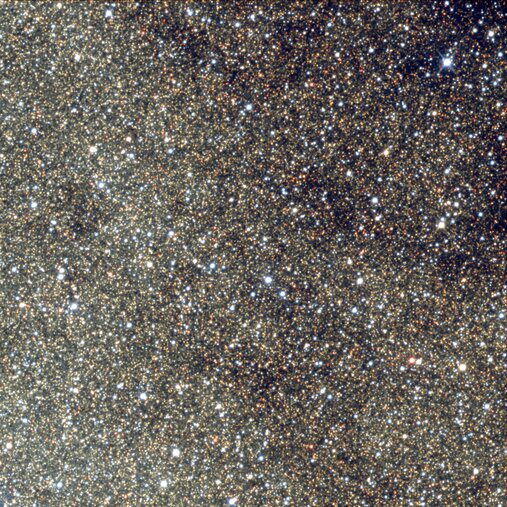
\includegraphics[width=0.5\linewidth]{static/microlensing/crowded_field.jpg}
        \caption{
            Stellar field of a microlensing event GLE-2012-BLG-0406 (centered),
            imaged by one of Las Cumbres Observatory's 2m telescopes,
            showing the high density of stars typical in microlensing observations.
            Credit: Y. Tsapras. Taken from
            \url{http://microlensing-source.org/pictures/}.}
        \label{fig:crowded_field}
    \end{centering}
\end{figure}

That the same effect could be used to detect the presence of planets orbiting
around the lens star was first theorized by \citet{1964PhRv..133..835L} who
wrote that \emph{``the primary effect of planetary deflectors bound to stars
    other than the Sun will be to slightly perturb the lens action of these
    stars''} although he was also sceptical about the possibility of detection,
saying that \emph{``associated pulses would be so weak and infrequent and of
    such fleeting duration – perhaps a few hours – as to defy detection''}.
Gravitational lensing as a method for discovering exoplanets really took off
with the work of Paczy\'nski
\citep{1986ApJ...304....1P,1986ApJ...301..503P,1991ApJ...374L..37M} who also
coined the term \emph{microlensing}, which refers to gravitational lensing in a
regime where the images of the background object cannot be resolved but one can
nevertheless measure its magnification as a function of time. Microlensing as a
method for detecting exoplanets has some unique aspects. First, it is a one-off
event which happens on a timescale of a few minutes up to several months
depending on the distances to the background star and the lensing star and the
mass of the lens. In addition to the fact that there's only one chance to
observe such an event for it to happen at all requires extremely precise
alignment between the lens and the background star and the chance of observing
a stellar microlensing event is about one-in-a-million (CITE) for a typical
star within the Milky Way. To observe a planetary signal is about an order of
magnitude less likely than that. Hence, obtaining a decent sample of planetary
events requires continuous monitoring on the order of $10^{8}$ stars at the
time which way microlensing observations that to focus on the densest region of
the Milky Way -- the galactic bulge. Figure~\ref{fig:crowded_field} a picture
from of such a dense stellar field. Finally, in the vast majority of cases we
do not detect any light from the lens itself, the collected photons are from a
background star completely unrelated and distant from the lensing star. This is
very different from other exoplanet discovery methods and it means that we only
obtain dynamical properties of planets such their masses and periods.

The aspects that make microlensing events that make them difficult to observe
also mean that it provides a unique lens onto exoplanet systems. Relative to
other methods such as transits and radial velocity, microlensing is sensitive
to planets located at substantially greater distances, well outside of our
Solar System neighborhood and even potentially to Milky Way's satellite
galaxies such as the Magellanic Clouds and the nearby Andromeda galaxy (CITE).
Microlensing is also sensitive to very to very small planets and planets which
are further out from the star than those typically detected using transits and
radial velocity. Microlensing surveys such as OGLE \citep{1993AcA....43..289U}
and MOA \citep{1999PThPS.133..233M} have been continuously monitoring crowded
stellar fields in the Milky Way since the 90s\footnote{Initially the focus was
    on finding dark matter candidate particles -- so called MACHOs (Massive Compact
    Halo Objects).} discovering thousands of stellar events and dozens of planetary
events. In order to detect planetary deviations in the observed light curve it
essential to have high cadence observations of the source star. The way surveys
have traditionally worked is that once a particular star started to become
magnified many additional small telescopes would start observing it to obtain
denser coverage and sometimes space-based observatories get involved as well.
The vast majority of microlensing events analyzed so far consist of
observations from multiple observatories, each with its own unique aspects such
as noise properties, cadence and photometric quality.

Future surveys such as the ground based Rubin Observatory
\citep{2019ApJ...873..111I} telescope and the space based Roman Telescope
\citep{2019ApJS..241....3P} and Euclid \citep{2022arXiv220209475B} will detect
tens of thousands of events in total. Although most of past work in the field
focused on characterizing individual events binary lens events, answering
questions about \emph{populations} with these new (but also existing) datasets
requires scalable data analysis methods and algorithms and a clear set of
guidelines on how to interpret the analysis products. This is a substantial
challenge because microlensing events are notoriously difficult to model. Even
though the datasets are relatively simple, consisting of multiple time series
photometric light curves in different bands, the parameter space of even the
simplest models is highly non-linear, correlated, relatively high dimensional
and there are often near perfect degeneracies in the solutions.

The assumptions that existing methods for modeling microlensing events rely on
are often opaque and unquestioned. Discussions on model ``degeneracies''
\citep{2014MNRAS.437.4006S,2019AJ....157...23H,2018AcA....68...43S,2009MNRAS.393..816D},
correlated noise \citep{2015ApJ...812..136B,2019MNRAS.488.3308L} and model
comparison \citep{2018AJ....155..259H,2019MNRAS.484.5608D} have been ongoing in
the microlensing literature for decades without a clear solution and proper
framing of the issue. In this thesis I will revisit these kinds of questions
while taking into account many recent developments in the fields of
computational statistics and machine learning. My main contributions are the
following:
\begin{itemize}
    \item I wrote an open-source Python package \textsf{caustics} which enables fast and
          accurate computation of binary and triple lens microlensing light curves using
          contour integration. The code runs on both CPU and GPU architectures, and
          crucially, for reasons that I will elaborate in subsequent chapters, it
          supports \emph{automatic differentiation} of all outputs with respect to all
          input parameters which enables the use of statistical methods which are orders
          of magnitude more efficient than existing approaches. The code can easily be
          extended to support quadruple lensing and arbitrary intensity profiles for the
          source star.
    \item I have revisited the topic of degeneracies in the posterior probability
          distributions which appear in the context of microlensing and propose solutions
          to these problems.
    \item I have extended the complex polynomial root solver from \citet{Cameron2021}
          such that it can be executed on GPU architectures and that it supports
          automatic differentiation. This enables the evaluation of ~1M lens equation
          solutions for point source binary and triple lenses in seconds using a CPU and
          miliseconds using a GPU.
    \item I propose an approach to statistical inference on a population of microlensing
          events which different from existing methods and has some advantages.
    \item I briefly discuss the issue of correlated noise in microlensing light curves
          and propose ways to account for it using Gaussian Processes.
\end{itemize}

\section{Occultation and phase curve mapping}
Interestingly, the second topic I will cover in this thesis has a history not
unlike that of microlensing. It was proposed in the early 20th century and it
was only much later that technology caught up with the idea. Back in 1906,
\citet{1906ApJ....24....1R} pointed out that certain features in light curves
of Solar System satellites may be attributed to inhomogeneities of their
surfaces. The key idea is that although at any given time we only observe the
total light from an unresolved satellite or planet, different portions of the
surface are visible at different times so we may expect that some of the
information about the surface intensity (be it emission from heat or reflected
Sunlight) gets imprinted onto the light curve. \citet{1906ApJ....24....1R} also
considered the inverse problem -- can we learn something about the surface of
these objects starting from a light curve? The method he proposed is now known
as \emph{phase curve mapping} and it was first attempted by
\citet{1972ApJ...174..449L} who analyzed photometric light curves of Pluto in
reflected light attempting to constrain variations in the \emph{albedo} of the
surface with inconclusive results.

Later works such as
\citet{1986AJ.....92.1201D,1992Icar...97..211B,1993Icar..102..134Y,1999AJ....117.1063Y}
went a step further by using not only phase curves but also light curves of
mutual \emph{occultations} of Pluto by its moon Charon to reconstruct albedo
maps with greater success. The major advantage of occultations relative to just
phase curves is that more information about the surface is encoded into the
light curve because of the sharp limb of the occultor sweeping over the disc of
an occulted body and blocking the reflected light. More importantly for this
thesis, \citet{1994Icar..107..195S} was the first to observe the occultations
of Jupiter's moon Io by another of Jupiter's moons -- Europa, and also
occultations of Io by Jupiter itself. These observations were conducted using
near-infrared telescopes such as NASA's Infrared Telescope Facility (IRTF) to
observe emitted light from Io's surface which is covered with many time-varying
and bright volcanic features. The observing campaign of Io has yielded insights
into the the nature of its volcanic activity and it continues to this day. I
will return to the subject of Io in great detail in
Chapter~\ref{ch:mapping_io}.

A natural question arises, can we do this with objects outside of the Solar
System? The answer is yes. \citet{2007Natur.447..183K},
\citet{2012ApJ...747L..20M}, and \citet{arXiv:1202.3829} used Spitzer
mid-infrared observations of secondary eclipses of the Hot Jupiter HD189733b
and found that surface emission is best described by the presence of a large
hot spot on the dayside of the planet which is longitudinally offset from the
substellar point. Similarly, \citet{2014Sci...346..838S}, produced temperature
maps of the Hot Jupiter WASP-43b, \citet{2013ApJ...776L..25D} mapped the Hot
Jupiter Kepler-7b in reflected light and \citet{2016Natur.532..207D} mapped the
thermal emission from the Super Earth 55 Cancri e. These studies were only able
to capture longitudinal variations in intensity. Real exoplanet atmospheres of
are certain to have three-dimensional spatial inhomogeneities in emission more
complex than a single hot spot due to the presence of clouds, zonal jets,
storms, waves etc. \citep{2020SSRv..216..139S}.

In recent years there have been significant advances in statistical modeling of
phase curves and eclipse light curves. Most notably,
\citet{2019AJ....157...64L} introduced the \textsf{starry} code which enables
analytic computation of phase curves and occultation light curves for bodies
with arbitrary emission maps expressed in a spherical harmonic basis (an idea
dating back to \citet{1906ApJ....24....1R} ) and \citet{2021arXiv210306275L}
expanded the algorithm for the (considerably more complicated) case of
reflected light. In this thesis, I will present the work I've done in
collaboration with other researchers from the planetary science and exoplanet
communities on using \textsf{starry} to map the surface of Io and investigate
the prospects for detecting fine spatial structure in the atmospheres of Hot
Jupiters using JWST phase curves and eclipse light curves. My contributions to
this area are the following:
\begin{itemize}
    \item I have developed a novel model for inferring emission maps of Io from
          occultation light curves. First part of this project is published in
          \citet{2022PSJ.....3...67B} though I haven't managed to complete the second
          part.
    \item I have investigated the problem of eclipse mapping of exoplanets using the
          \textsf{starry} framework, focusing in particular on the possibility of
          detecting planetary scale storms on Hot Jupiters using JWST. I found that it
          extremely difficult to infer maps of higher resolution than a dipole order but
          that should still be sufficient for detecting large scale weather and climate
          change in the atmospheres of these planets.
\end{itemize}
The application of the occultation/eclipse mapping method to Io can be seen as the
best case scenario for the application of the same method to exoplanets.
I will show that even in the case of observing a bright object right in our neighborhood,
this is by no means and easy task. Our ability to reconstruct the surface features of
Io sets a sort of upper limit on what is possible with exoplanets.

%\section{Outline}
%The outline of the thesis is as follows. Chapter~\ref{ch:theoretical_min}
%contains the theoretical background needed to understand the subsequent
%chapters, covering the theory behind microlensing and occultation mapping, a
%summary of Bayesian statistics in particular and statistical inference more
%generally, and probabilistic programming which ties everything together.
%Chapter~\ref{ch:microlensing} is the most extensive chapter in the thesis
%covering all of my work on microlensing. I start by discussing the case of
%single lens microlensing models, showing that it contains many of the
%properties of more complex models. In particular I focus on the issue of
%multi-modal posterior distributions which is a ubiquitous problem in
%microlensing. I propose several solutions to this and demonstrate their
%effectiveness. I then move on to the considerably more complex case of binary
%and triple lens models starting with numerical methods for solving the lens
%equation (finding roots of a complex polynomial equation). I demonstrate the
%advantage of the Ehrlich-Aberth algorithm over previous methods and explain how
%to make this algorithm differentiable and orders of magnitude faster through
%the use of GPUs. Next, I cover the contour integration algorithm for computing
%the magnification of a limb-darkened source star and its implementation in
%\textsf{caustics}.

% CHAPTER 2: The theoretical minimum
\chapter{The theoretical minimum}
\label{ch:theoretical_min}

\section{Gravitational microlensing}
\label{sec:microlensing}
Gravitational lensing is generally divided into multiple classes depending
on weather the effect is discernible at the level of individual objects or a
a statistical sample of object. The main division is between \emph{weak lensing}
and \emph{strong lensing}.
The former refers to lensing by galaxies and clusters of galaxies on cosmological
scales where the deflection  is impossible to detect in a single background source
but one can tease out the effect in a statistical sense.
Strong lensing refers to lensing of individual objects and it is further divided into
\emph{macrolensing} -- lensing of galaxies where the multiple images of the source
are resolved, and \emph{microlensing}  -- the images are generally not resolved,
and the observable is the total magnification of the source as a function of time (a light curve).
In case of microlensing the light source is either a quasar or a star (sometimes a binary star)
and the lenses are stars, brown dwarfs, planets, and compact objects such as black holes, neutron
stars and white dwarfs. In this thesis we focus specifically on microlensing
with stars as the light source instead of quasars\footnote{Quasar microlensing
    is a somewhat separate community from the rest of the microlensing community.}.

\subsection{Deflection of light by gravity}
Gravitational lensing is a phenomenon fully described by Einstein's General
Theory of Relativity (GR) in which light changes its direction of propagation
when passing close to a massive body. GR predicts the following:
\begin{itemize}
    \item the presences of mass changes the spacetime geometry from the flat (Minkowski)
          metric $\eta_{\mu\nu}$ to a curved metric, specified by the tensor $g_{\mu\nu}$
    \item massless particles such as photons follow the null geodesics -- minimum
          distance paths in curved spacetime which are obtained by solving the
          \emph{geodesic equation}
\end{itemize}
If we restrict ourselves to the regime where the metric is time independent
and the particles are allowed to travel at any velocity less than $c$,
also known as the \emph{weak field} or \emph{linearized approximation }
of GR, the metric tensor
can be written as
\begin{equation}
    g_{\mu\nu}=\eta_{\mu\nu}+h_{\mu\nu}\quad,
\end{equation}
where $h_{\mu\nu}=
    \textrm{diag}(-2\Phi,-2\Phi,-2\Phi,-2\Phi)$\footnote{Assuming the
    the metric sign convention $(-,+,+,+)$} \citep{carroll_2019}.
The (static) Newtonian gravitational potential $\Phi$ obeys the Poisson equation
\begin{equation}
    \nabla^2\Phi=4\pi G\rho\quad,
\end{equation}
where $\rho$ is the mass density of the distribution of mass located between the observer
and the light source.
The geometry of the lensing system consisting of a distant source of light, the
observer, and a distribution of mass with density $\rho$ located between the
source and the observer is shown in Figure~\ref{fig:deflection_angle}.
\begin{figure}
    \centering
    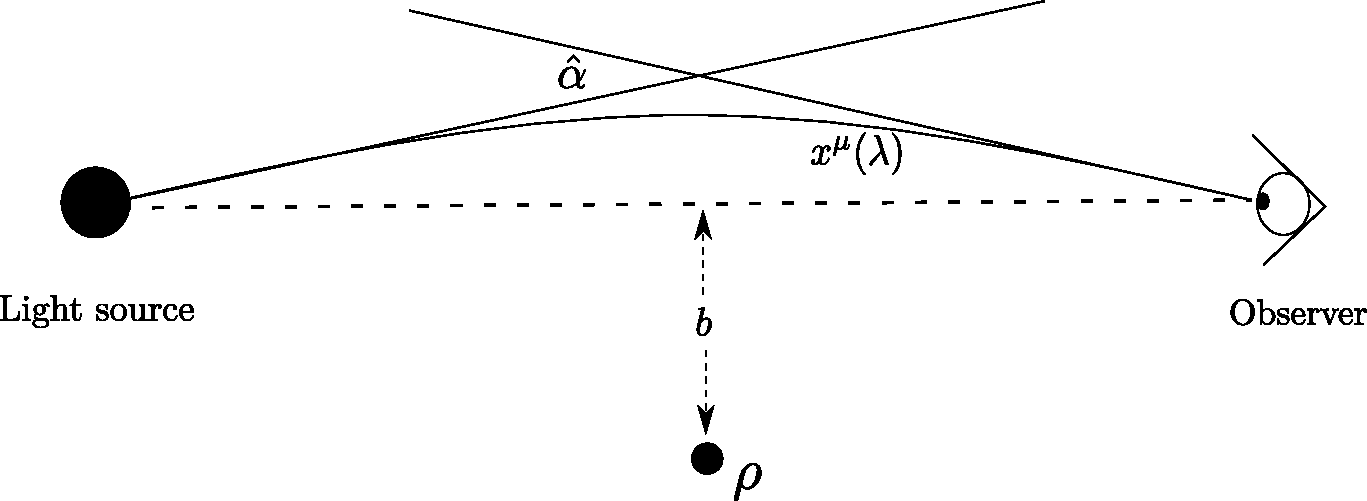
\includegraphics[width=0.6\linewidth]{static/microlensing/deflection_angle.pdf}
    \caption{Geometry of gravitational lensing.
        A geodesic curve $x^\mu(\lambda)$ is deflected
        by an angle $\hat\alpha$ from its initial trajectory
        due to the presence of a massive body with mass density $\rho$. Figure
        adapted from \citet{carroll_2019}.}
    \label{fig:deflection_angle}
\end{figure}
A photon is deflected as it travels from a source to an observer by a
\emph{deflection angle} $\hat\alpha$, a vector in the
plane  perpendicular to the wave vector $\vec{k}$ pointing in the direction of
photon propagation.
The deflection angle is given by \citep{carroll_2019}
\begin{equation}
    \hat\alpha=2\int\nabla_\perp\Phi \ud s\quad,
    \label{eq:deflection_angle_general}
\end{equation}
where $\nabla_\perp\Phi$ is the gradient of the potential in the direction transverse
to the path of the photon and $s$ is the spatial distance traveled.
For a point mass $M$, the potential is given by the potential is
\begin{equation}
    \Phi=- \frac{GM}{(b^2+x^2)^{1/2}}\quad,
\end{equation}
where $x$ parametrizes the straight line distance between the observer and the lens and
$b$ is the impact parameter of the light ray.
Integrating from $-\infty$ to $\infty$ (i.e. assuming that both
the source and the observer are located far away from the deflecting mass), we obtain
the deflection angle:
\begin{equation}
    \hat\alpha= \frac{4GM}{c^2b}= \frac{2R_s}{b}\quad,
\end{equation}
where $R_s=2GM/c^2$ is the Schwarzschild radius.
$\hat\alpha$ is directly proportional to the mass of the lens and
it does not depend on the wavelength of the light. It also increases with the proximity of
the light ray to the lensing mass which is the opposite behavior to that of a
classical convex lens for which the deflection angle vanishes at the center of the lens.
The gravitational lens does not have a focal length and so it is not a lens in the usual
sense.
The resulting deflection angle is very small, for example, for the Sun we have
$GM/c^2=1.48\times 10^5\si{\centi\meter}$ (2.95 km), $R=6.96\times
    10^{10}\si{\centi\meter}$ and $\hat\alpha=1.75$ arc seconds. This is the angle
that was claimed to have been observed by Eddington when during the 1919 total
solar eclipse.

Equation~\ref{eq:deflection_angle_general} is only valid when the linearized
approximation of GR is sufficient. In this approximation, the deflection angles
are additive and the total deflection caused by a group massive bodies is just
the sum of the individual deflection angles. The linearized approximation
breaks down when the impact parameter $b$ approaches the Schwarzschild radius
of the lensing mass and the linearized metric is no longer sufficient. Except
for modeling lensing in the close vicinity of a black, the linearized
approximation is sufficient.

\subsection{The magnification of a point source by a point lens}
Consider a system consisting of an observer $O$, a point mass $M$, and a point
light source $S$. The geometry of this system is shown in
Figure~\ref{fig:lens_geometry}. The lens is located in the \emph{lens plane}, a
plane perpendicular to the observer--lens axis, at a distance $D_L$ away from
the source. The light source is located in the \emph{source plane}
perpendicular to the observer--source axis, at a distance $D_S$ away from the
observer, and the observer is in the \emph{observer plane}. The assumption that
the location of the source, observer, and the lens can be parametrized using
angular coordinates (or Cartesian coordinates if the distances to the lens and
the source are known) in their respective planes is justifiable because the
deflection angles involved are very small and the distance between the observer
and any point of interest in the lens plane is approximately constant.
\begin{figure}[!ht]
    \centering
    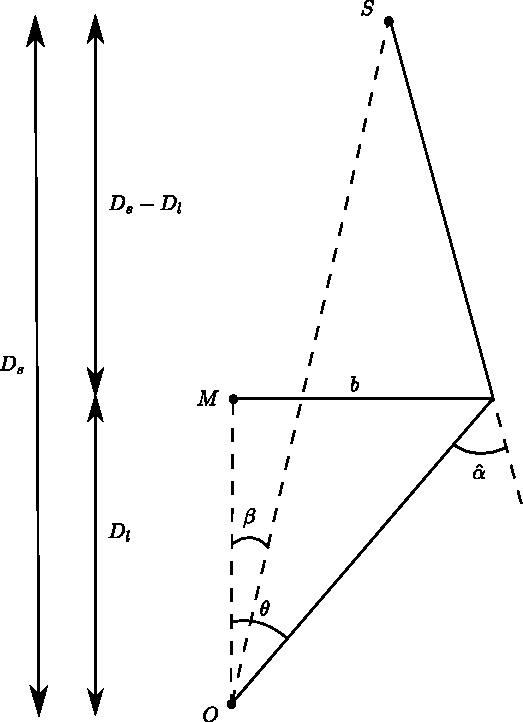
\includegraphics[width=0.4\linewidth]{static/microlensing/lens_geometry.pdf}
    \caption{The geometry of a system consisting of a point mass lens $M$ located at distance
        $D_L$ at angular separation $\beta$ from the observer, and a single light source $S$ located at distance $D_S$, emitting a light ray which gets
        deflected by an angle $\hat\alpha$ from its
        original trajectory. As a result the observer sees the source at angular separation
        $\theta$. Figure adapted from \citet{1992grle.book.....S}.}

    \label{fig:lens_geometry}
\end{figure}
Let $\theta$ be the apparent angular position of the source in the sky with respect to the
observer--lens axis and $\beta$ be the actual angular position of the source.
Assuming a metric for spacetime in between the source and the observer that is
approximately Euclidian\footnote{This is a valid assumption for galactic sources but not for
    extragalactric source such as quasars and galaxies which require a cosmological
    model for the metric.} the distance from the lens to the
source is $D_S-D_L$.

From Figure~\ref{fig:lens_geometry} it follows that the relationship between
the observed and the actual location of the source is given by
\begin{equation}
    \beta=\theta-2 R_s \frac{D_S-D_L}{D_LD_S}
    \frac{1}{\theta}\quad,
    \label{eq:lens_equation}
\end{equation}
which is known as the \emph{lens equation} or sometimes also the \emph{ray-tracing}
equation. If the source and the lens are perfectly aligned with respect to the observer,
then $\beta=0$ and $\theta\equiv\theta_E$ where
\begin{equation}
    \theta_E= \sqrt{ \frac{4GM}{c^2} \left( \frac{1}{D_L} - \frac{1}{D_S} \right)}=
    \sqrt{\kappa M\pi_{LS}}
    \label{eq:angular_einstein_radius}
\end{equation}
where $\kappa \equiv \frac{4 G}{c^{2} \mathrm{au}} \simeq 8.1 \frac{\mathrm{mas}}{M_{\odot}}$
and
\begin{equation}
    \pi_{LS}\equiv\pi_L - \pi_S=\frac{1\mathrm{au}}{D_L}-\frac{1\mathrm{au}}{D_S}
\end{equation}
is the relative lens-source parallax.

The image of the source forms a ring (the Einstein ring) around the lens star
with angular radius $\theta_E$ -- the \emph{Einstein radius}. $\theta_E$
depends on the mass of the lens and the distances to the lens and the source.
The angular Einstein radius sets the characteristic scale of a microlensing
event, it is a natural unit for most microlensing parameters. For an M-dwarf
star lens in the galactic disc ($D_L\sim 3\,\textrm{kpc}$) and a source star in
the galactic bulge ($D_S\sim 8\,\textrm{kpc}$) we have $\theta_E\sim
    1\,\textrm{mas}$ so the typical scale of microlensing is on the order of
miliarcseconds. The images of the source star are only rarely observable using
the most advanced optical interferometers such as the GRAVITY instrument on
ESO's Very Large Telescope whose lower resolution limit is $2\,\textrm{mas}$
\citep{arXiv:1705.02345}. \cite{2019ApJ...871...70D} were the first to resolve
the images of a microlensing event, finding the value of
$\theta_E=1.87\,\textrm{mas}$ using the GRAVITY instrument.

We can rewrite Equation~\ref{eq:lens_equation} by defining new dimensionless
angular coordinates scaled by the angular Einstein radius:
\begin{equation}
    x= \frac{\theta}{D_L\theta_E}, \quad y=\frac{\beta}{D_S\theta_E}
\end{equation}
The lens equation then takes the very simple form
\begin{equation}
    y= x- \frac{ 1}{x}
    \label{eq:lens_equation_dimensionless}
\end{equation}
Equation~\ref{eq:lens_equation_dimensionless} is a nonlinear mapping between the
source plane $y$ and the image plane $x$.
If we solve for $x$, we obtain two solutions for the position of the images, given by

\begin{equation}
    x_\pm= \frac{1}{2} \left( y\pm\sqrt{y^2 +4}\right)
    \label{eq:images_location}
\end{equation}
For non zero $y$ the so called \emph{minor image} is always located
within the Einstein radius ($\lvert x_-\rvert<1$) while the \emph{major image}
is located outside of it ($\lvert x_+\rvert>1$).

Since gravitational lensing does not involve any additional emission or
absorption along a deflected ray of light and since the wavelength of the light
ray does not change when it encounters the lens, the \emph{surface brightness}
(flux density per unit angular area) $I$ of the source image is identical to
the surface brightness of the unlensed source. The flux of an infinitesimal
source is a product of the surface brightness and the solid angle $\Delta
    \omega$ subtended by the source in the sky which changes throughout the
microlensing event because the source and the lens are in motion relative to an
observer. The ratio of the original and the lensed source flux, the
\emph{magnification} $A$, is then given by the ratio of the two solid angles
\begin{equation}
    A= \frac{\Delta \omega}{(\Delta\omega)_0}\quad,
    \label{eq:magnification}
\end{equation}
where $0$ denotes the unlensed solid angle.
Assuming an infinitesimal source size at angular location $\mathbf y =(y_1,y_2)$ subtending an angle
$\Delta (\omega)_0$, and an image of the source at location $\mathbf x=(x_1,x_2)$ subtending an angle
$\Delta \omega$; the ratio between the solid angle of the source and the image
is given by the determinant of the Jacobian matrix of the
lens mapping $\mathbf{x}\rightarrow\mathbf{y}$, evaluated at the location of the images
\begin{equation}
    \frac{(\Delta\omega)_0}{\Delta\omega} =\left\lvert\textrm{det}
    \frac{\partial \mathbf y}{\partial \mathbf x} \right\rvert
\end{equation}
The magnification $A$ is then given by the inverse Jacobian determinant of the lens mapping:
\begin{equation}
    A= \left\lvert\det
    \frac{\partial \mathbf y}{\partial \mathbf x} \right\rvert^{-1} \label{eq:magnification_general}
\end{equation}
The images for which the determinant of the Jacobian of the lens mapping is
positive are said to have positive \emph{parity} and vice versa.

Looking at Equation~\ref{eq:magnification_general}, we see that the
magnification diverges when the Jacobian determinant of the lens mapping
vanishes. Curves in the lens plane for which the determinant of the lens
mapping vanishes, that is,
\begin{equation}
    \left\lvert\det
    \frac{\partial \mathbf y}{\partial \mathbf x} \right\rvert=0
\end{equation}
are called \emph{critical curves}.
The critical curves in the lens plane can be mapped to the source plane using
the lens equation $\mathbf{x}\rightarrow \mathbf{y}$ and these curves are
are called \emph{caustic curves}.
Although the magnification factor in Equation~\ref{eq:magnification_general} formally
diverges at the points of critical curves or caustics,
the divergence is not physical because light sources aren't truly point like.
If the finite angular size of the source is taken into
account, the magnification is an integral of Equation~\ref{eq:magnification_general} over the
extent of the source, weighted by the source brightness and that integral is always finite.
Both the critical and the caustic curves are closed and one can prove that \textbf{the
    number of images changes by two if and only if the source crosses a caustic curve}
\citep[][Chapter 6]{1992grle.book.....S}.

We can derive a simpler expression for Equation~\ref{eq:magnification} by
switching to polar coordinates $(v,\phi)$ in the lens plane. The lens equation
for the two vector components of the apparent source position is given by
\begin{align}
    y_1= & x_1- \frac{x_1}{x_1^2+x_2^2} \\
    y_2= & x_2- \frac{x_2}{x_1^2+x_2^2}
\end{align}
Introducing polar coordinates $x_1=v\cos\phi,\;x_2=v\sin\phi$, we have
\begin{equation}
    \left\lvert\textrm{det}
    \frac{\partial \mathbf y}{\partial \mathbf x} \right\rvert =1- \frac{1}{v^4}\quad,
\end{equation}
By substituting in the locations of the source images Equation~\ref{eq:images_location} into the
above expression, we obtain the magnification of the source for both images
\begin{equation}
    A_\pm=\left(1- \frac{1}{x^4_\pm} \right)^{-1}
\end{equation}
The total magnification is then the sum of the two magnifications, and is given by
\citep{1936Sci....84..506E}
\begin{equation}
    A(u)=\lvert A_-\rvert+\lvert A_+\rvert= \frac{u^2+2}{u\sqrt{u^2+4}}\quad,
    \label{eq:magnification_point_lens}
\end{equation}
where $u = \sqrt{y_1^2+y_2^2}$ is the the magnitude of the position
vector of the source star.
The critical curve of the point lens is the Einstein
ring corresponding to $v=\sqrt{x_1^2+x_2^2}=1$ and the caustic curve is mapped to a
a single point in the source plane at $u=0$.
For source separations much smaller than the angular Einstein radius ($u\ll 1$), the
magnification is approximately $A(u)\simeq 1/u$, in the opposite case ($u\gg 1$)
we have $A(u)\simeq 1+ 2/u^4$, that is, the magnification falls off rapidly the further
away the source is from the lens.

To be able to evaluate Equation~\ref{eq:magnification_point_lens} in practice
we have to parametrize the position of the source on the sky $u$ as a function
of time. To derive an expression for $u(t)$ we assume the the motion of the
observer, lens and the source is rectilinear (acceleration can be neglected).
We take $\vec{x}_S$ to be the angular position of the source star on the plane
of the sky and $\boldsymbol{\mu}_L$ to be its proper motion vector. Likewise
for the lens. We thus have
\begin{align}
    \vec{x}_S(t) & =\vec{x}_{S, 0}+
    \left(t-t_{0}\right) \boldsymbol{\mu}_S
    \label{eq:source_position}      \\
    \vec{x}_L(t) & =\vec{x}_{L, 0}
    +\left(t-t_{0}\right) \boldsymbol{\mu}_L\quad,
    \label{eq:lens_position}
\end{align}
where $t_0$ is some reference time.
The relative position vector of the lens with respect to the source is then
\begin{equation}
    \boldsymbol{u}(t) \equiv \frac{\vec{x}_L(t)
        -\vec{x}_S(t)}{\theta_E}=
    \frac{\vec{x}_{LS, 0}}{\theta_E}
    +\frac{t-t_{0}}{\theta_E} \boldsymbol{\mu}_{LS}
    \label{eq:relative_trajectory_no_parallax}
\end{equation}
where
$\vec{x}_{L S, 0}\equiv\vec{x}_{L,0}-\vec{x}_{S, 0}$
is the relative position at $t_0$ and
$\boldsymbol{\mu}_{LS}\equiv \boldsymbol{\mu}_{L}- \boldsymbol{\mu}_{S}$ is the
relative proper motion.
Since $\boldsymbol{\mu}_{LS}$ and $\vec{x}_{L S, 0}$ are
perpendicular to each other, it follows that the magnitude of the relative
separation is
\begin{equation}
    u(t)=\sqrt{u_0^2+ \left(\frac{t-t_0}{t_E}\right)^2}
\end{equation}
where we have defined $u_0\equiv |\vec{x}_{L S, 0}|/\theta_E$
and $t_E\equiv \theta_E/|\boldsymbol{\mu}_{LS}|$.
The magnification is then a function of three parameters $(t_0, u_0, t_E)$
and the resulting curve as a function of time is often called the Paczy\'nski curve
\citep{1986ApJ...304....1P,1986ApJ...301..503P}.
The magnification as a function of time for different impact parameters $u_0$
is shown in Figure~\ref{fig:paczynski_curve}. Notice the very steep fall off in
magnification as as we move away from the Einstein ring ($A(u)\propto
    1+2u^{-4}$).
In the limits of $u_0\rightarrow 0$ and $u_0\gg 1$  there is a continuous
mathematical degeneracy between the parameters $t_0$, $u_0$ and $t_E$
\citep{1997ApJ...487...55W}.

\begin{figure}[t]
    \begin{centering}
        \includegraphics[width=0.7\linewidth]{figures/paczynski_curve.pdf}
        \caption{
            Magnification of a point source by a point lens as a function of time. The
            various magnification curves correspond to different impact parameters $u_0$.
            The inset figure
            shows the source trajectories in the lens plane, the dashed circle corresponds
            to the Einstein radius $v=1$.}
        \label{fig:paczynski_curve}
    \end{centering}
\end{figure}

\subsection{Observed flux}
The magnification $A(t)$ is not a direct observable in microlensing events. We
can only measure the flux of the source star which is usually contaminated with
the flux of other nearby stars in the dense stellar field and potentially also
with light from the lens and possible companions to the lens. The observed flux
is thus given by
\begin{equation}
    F(t)=F_S(t)+F_B(t)
    \label{eq:flux_observed}
\end{equation}
where $F_s$ is the flux of the source star and $F_B$ is the contamination flux also
called the \emph{blending flux}. To quantify the strength of the blending e can
define the emph{source flux fraction} $b_S$ as the fraction of total (unmagnified)
flux that is coming from the source star:
\begin{equation}
    b_S\equiv F_S/(F_S + F_B)
\end{equation}
For highly blended events $b_S\approx 0$ and in absence of blending $b_S=1$.
The source flux $F_S$ and the blending flux $F_B$ are generally highly correlated
and it is often preferable to use a slightly different parametrization proposed by
\citet{2009MNRAS.393..816D}. In this parametrization we use the
\emph{baseline flux} $F_\mathrm{base}$ and the difference between
the baseline flux and the flux at peak magnification $\Delta F\equiv F_S[A(u_0)-1]$
as the new parameters.
Equation~\ref{eq:flux_observed} then takes the form
\begin{equation}
    f=\Delta F\frac{A(t) - 1}{A(t_0)-1}+F_\mathrm{base}
    \label{eq:flux_dominik}
\end{equation}
It is generally straightforward to measure the flux difference $\Delta F$, the
baseline flux $F_\mathrm{base}$ and the center of the curve $t_0$ but getting a
good estimate of $t_E$ even outside of the regime $u_0\rightarrow 0$ and
$u_0\gg 1$ requires good photometric sampling along the ``wings'' of the light
curve \citep{2009MNRAS.393..816D}.

\subsection{Magnification of an extended source}
\begin{figure}[t]
    \begin{centering}
        \includegraphics[width=\linewidth]{figures/single_lens_images.pdf}
        \caption{Images of an extended limb-darkened source star lensed by a single
            point lens for varying position of the source star. The top panels show the magnification map with a logarithmic scale
            colormap  consisting of a single point caustic. The semi-transparent circle
            is the source star disc with radius $\rho_\star=0.15$. The bottom row shows
            the two images merging into the Einstein ring as the source moves over the caustic.}
        \label{fig:single_lens_images}
    \end{centering}
\end{figure}
For a relatively small subset of microlensing events the source star passes
very close to the caustic and the variation of magnification over the extent of
the source star disc is non-negligible. For those events the point source
approximation breaks down and we have to take into account the finite angular
radius $\theta_\star$. This will generally happen when $u_0 \lesssim
    \rho_\star/2$ \citep{1997ApJ...477..580G} where
$\rho_\star=\theta_\star/\theta_E$. The effect of finite source effects on the
magnification curve thus matters only near the peak of an event and it results
in a rounder top of the curves shown in Figure~\ref{fig:paczynski_curve}.
Unfortunately there are no analytic solutions for the magnification of an
extended source lensed by a single point lens with a general surface brightness
profile. \citet{1994ApJ...421L..71G} derived an approximate solution valid for
uniform brightness sources with $\rho_\star\lesssim 0.1$ and
\citet{1994ApJ...430..505W} derived a general solution (also for a uniform
brightness source) involving solutions to elliptic integrals of the first,
second and third kind. A general solution involving Fast Fourier Transforms
which is applicable to any source profile was recently proposed by
\citet{2022arXiv220306637S}.

In Figure~\ref{fig:single_lens_images} we show the magnification map and the
images of an extended limb-darkened source with $\rho_\star=0.15$ as it
approaches the point caustic for a single lens. The top panels show the
magnification map in the source plane using a logarithmic scale colormap. The
source disc is shown (semi-transparent grey circle) at different positions
relative to the caustic. The bottom panels show the resulting images in the
image plane, this is what we would see on the sky if we could resolve the
microlensing event. As the source moves closer to the caustic the area (and
hence the magnification) of the two images increases and eventually they merge
forming an Einstein ring.

To produce these plots I evaluated the lens mapping
(Eq.~\ref{eq:lens_equation_dimensionless}) on a regular grid in the image plane
and then plotted the surface brightness of the corresponding point on the
source disc in the source plane. I will discuss all of this in far greater
detail In Chapter~\ref{ch:microlensing} but for now I should mention a few key
points:
\begin{itemize}
    \item Every point inside the two images maps to a single point on the source disc via
          the lens equation. The inverse mapping is one-to-many because each point on the
          source disc maps to two points (point lens images) in the image plane. The
          points on the limbs of the two images correspond to the points on the limb of
          the source disc. We cannot predict the location of the images without inverting
          the lens mapping
    \item To numerically compute the magnification of an extended source, we could either
          integrate the magnification function convolved with the source brightness
          profile over the entire source disc (a two-dimensional integral), or we could
          do the same integral in the image plane. The first approach is highly
          numerically unstable because we would need to integrate over a function which
          diverges as $1/r$ approaching the caustic and this would require a very large
          number of lens equation evaluations. Hence it is much better to integrate in
          the image plane where the function is smooth.
    \item Decreasing the source radius $\rho_\star$ results in narrower arcs of the
          images (smaller radial extent).
\end{itemize}

\subsection{Annual parallax}
\label{ssec:single_lens_parallax}
In Equation~\ref{eq:relative_trajectory_no_parallax} we have assumed that the
relative motion of the lens with respect to the source on the plane of the sky
is rectilinear.
This is a reasonable approximation in a barycentric frame of
reference if the acceleration of the source and the lens can be neglected.
However, most microlensing events are observed from a non-inertial geocentric
frame (Earth) and sometimes also from multiple locations simultaneously. In those
cases we have to take into account parallax effects.
We differentiate between two kinds of parallax. First is the \emph{annual
    parallax} (sometimes also called the orbital parallax) which modifies the
lens-source relative motion vector $\boldsymbol\mu_{LS}$ due to the local
acceleration of Earth in its orbit. It is important for long timescale events
when the event timescale is equal to some substantial fraction of a year. The
effect of annual parallax is usually a slight modification of the shape of the
Paczy\'nski curve.

The second kind of parallax is the \emph{satellite parallax} which refers to a
difference in viewpoint when conducting simultaneous observations of the source
star from different locations separated by a substantial fraction of the
Einstein ring projected onto the observer plane $\tilde{r}_E\equiv
    D_{LS}\theta_E$ (where $D_{LS}^{-1}=D_L^{-1} - D_S^{-1}$). In practice this
means observing a microlensing event from Earth and a space based telescope
simultaneously. It was first proposed by \citet{1966MNRAS.134..315R}. There is
also the ``terrestrial parallax'' which is identical to the satellite parallax
except that it involves only ground-based observations separated by a large
fraction of Earth's diameter. A measurement of these parallax effects allows
for a partial breaking of the degeneracy in the event timescale $t_E$ by
providing a relationship between the mass and the distance to the lens
(assuming one can estimate the distance to the source star).

In this section I will describe the annual parallax effect. We start by
modifying Equations~\ref{eq:source_position} and \ref{eq:lens_position} to
include the projected motion of the Sun relative to the Earth on the plane of
the sky. We project $\mathbf s$ -- the position vector of the Sun relative to
Earth, onto a plane perpendicular to the line of sight towards the source star
(plane of the sky) which is defined by the unit vector $\boldsymbol{\hat n}$
normal to the plane. The unit vector $\boldsymbol{\hat n}$ depends on the sky
coordinates of the source star $(\alpha,\delta)$ (right ascension and
declination). We choose to work in geocentric equatorial coordinates defined by
the spherical unit vectors $\hat{\mathbf e}_n$, pointing North, and
$\hat{\mathbf e}_e$ pointing eastward such that the coordinate system is
right-handed. The unit vectors are defined by
\begin{align}
    \hat{\mathbf e}_e & = \hat{\mathbf z}\times \hat{\mathbf n}  \\
    \hat{\mathbf e}_n & = \hat{\mathbf n}\times\hat{\mathbf e}_e
\end{align}
The two components of $\mathbf s$ projected onto the plane of the sky are then
\begin{align}
    \zeta_e(t;\alpha,\delta)\equiv \mathbf s\cdot \hat{\mathbf e}_e \\
    \zeta_n(t;\alpha,\delta)\equiv \mathbf s\cdot \hat{\mathbf e}_n
\end{align}
In practice, we can retrieve $\mathbf{s}$ using NASA's JPL Horizons system and compute
the projected separation at any time $t$.
The angular positions of the source and the lens
(Equations~\ref{eq:source_position} and \ref{eq:lens_position}) then become
\begin{align}
    \vec{x}_S(t) & = \vec{x}_{S,0}+(t-t_0)\boldsymbol{\mu}_S
    +\pi_S\,\boldsymbol{\zeta}(t)                            \\
    \vec{x}_L(t) & = \vec{x}_{L,0}+(t-t_0)\boldsymbol{\mu}_L
    +\pi_L\,\boldsymbol{\zeta}(t)
\end{align}
where  $\pi_S\equiv 1\,\mathrm{au}/D_S$ is the source parallax, and $\pi_L$ is the
lens parallax.
The relative separation is then
\begin{equation}
    \boldsymbol{u}(t)= \frac{\boldsymbol\theta_{LS, 0}}{\theta_E}
    +\frac{t-t_0}{\theta_E}\boldsymbol{\mu}_{LS}+\pi_{E}\,\boldsymbol{\zeta}(t)
    \label{eq:relative_separation_parallax}
\end{equation}
where
\begin{equation}
    \pi_E\equiv \frac{\pi_{LS}}{\theta_E}
    \label{eq:pi_E}
\end{equation}

Since annual parallax is a higher order effect affecting the apparent
trajectory of the source on the sky, it makes sense to decompose the trajectory
as a sum of rectilinear motion plus a deviation due to parallax. Following
\citet{2004ApJ...606..319G} we define the position offset of the Sun on the
plane of the sky relative to its position at a particular time $t_0'$ as

\begin{equation}
    \delta\boldsymbol \zeta (t)=\boldsymbol \zeta (t)-\boldsymbol \zeta (t_0')-(t-t_0')
    \boldsymbol{\dot \zeta} (t_0')
\end{equation}
By construction, we have $\delta\boldsymbol \zeta (t_0')=0$ and
$\delta\dot{\boldsymbol \zeta} (t_0')=0$.
Equation~\ref{eq:relative_separation_parallax} then takes the form
\begin{equation}
    \boldsymbol{u}(t)=\mathbf{u}_0 + (t-t_0')\,\dot{\mathbf{u}}_0 +
    \pi_E\,\delta\boldsymbol \zeta(t)
    \label{eq:relative_separation_parallax_decomposed}
\end{equation}
where
\begin{align}
    \mathbf{u}_0       & \equiv \mathbf{u}(t_0) =\frac{\boldsymbol\theta_{LS, 0}}{\theta_E}
    + \frac{(t_0'-t_0)}{\theta_E}\boldsymbol\mu_{LS}+
    \pi_E\,\boldsymbol \zeta(t_0)                                                           \\
    \dot{\mathbf{u}}_0 & \equiv\dot{\mathbf{u}}(t_0)=
    \frac{\boldsymbol\mu_{LS}}{\theta_E}  + \pi_E\,\dot{\boldsymbol \zeta}
    (t_0')
\end{align}
In what follows, we set the reference time to $t_0'\equiv t_0$ in order to ensure that
the vectors $\mathbf{u}_0$ and $\dot{\mathbf{u}}_0$ are perpendicular to each other,
which is the case at $t=t_0$ because at $t_0$ the trajectory has a local extremum
\footnote{In CITE, $t_0'$ is fixed to a particular value. It is not clear
    to me how this ensures that the two vectors are perpendicular to each other
    (TODO: show that this is true).}

\subsubsection{$\mathbf{u}(t)$ in the $(\mathbf{\hat e}_\bot,
        \mathbf{\hat e}_\parallel)$ coordinate system}%

\begin{figure}
    \centering
    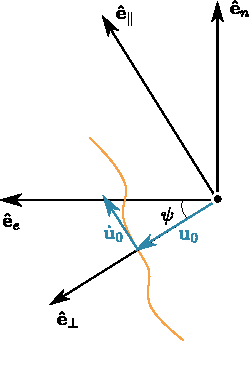
\includegraphics[width=0.3\linewidth]{static/microlensing/microlensing_parallax_coordinates.pdf}
    \caption{A coordinate system
        $(\mathbf{\hat e}_\bot,\mathbf{\hat e}_\parallel)$ parallel to the source trajectory at time $t_0$. The orange curve
        represents the source trajectory relative to the lens at the origin. The
        coordinate system $(\mathbf{\hat e}_\bot,\mathbf{\hat e}_\parallel)$ is related to the equatorial coordinates $(\mathbf{\hat
                e}_e,\mathbf{\hat e}_n)$ by a rotation through an angle $\psi$.}
    \label{fig:parallax2}
\end{figure}

To evaluate Equation~\ref{eq:relative_separation_parallax_decomposed}, we need
to choose a suitable basis. A natural coordinate system for describing the
trajectory of the source relative to the lens is one defined by unit vectors
$(\mathbf{\hat e}_\bot,\mathbf{\hat e}_\parallel)$ where $\mathbf{\hat e}_\parallel$ is parallel to the trajectory $\mathbf{u}(t)$ at time $t_0$
(Figure~\ref{fig:parallax2}). We define the unit vectors as
\begin{equation}
    \mathbf{\hat e}_\bot\equiv \frac{\mathbf{u}_0}{|\mathbf{u}_0|}\quad,
    \mathbf{\hat e}_\parallel\equiv \frac{\mathbf{\hat n}\times\mathbf{u}_0}{|\mathbf{u}_0|}\quad
\end{equation}
and the coordinate system $(\mathbf{\hat e}_\bot,\mathbf{\hat e}_\parallel)$ is related to ecliptic coordinates via a simple rotation through an
angle $\psi$
\begin{equation}
    \begin{pmatrix}
        \mathbf{\hat e}_\bot \\
        \mathbf{\hat e}_\parallel
    \end{pmatrix}
    =
    \begin{pmatrix}
        \cos\psi & -\sin\psi \\
        \sin\psi & \cos\psi
    \end{pmatrix}
    \begin{pmatrix}
        \mathbf{\hat e}_e \\
        \mathbf{\hat e}_n
    \end{pmatrix}
    \label{eq:ecliptic_to_parallel}
\end{equation}
By construction, at time $t_0$ we have
$\mathbf{u}_0\,\bot\,\dot{\mathbf{u}}_0$ and the two components of
$\mathbf{u}(t)$ are then
\begin{align}
    u_\bot(t)      & \equiv \mathbf{u}(t)\cdot \mathbf{\hat e}_\bot= u_0 +
    \pi_E\,\delta\boldsymbol \zeta(t)\cdot\mathbf{\hat e}_\bot                                                                                                                                       \\
    u_\parallel(t) & \equiv \mathbf{u}(t)\cdot \mathbf{\hat e}_\parallel= (t-t_0)\,\dot{\mathbf{u}}_0\cdot\mathbf{\hat e}_\parallel+ \pi_E\,\delta\boldsymbol \zeta(t)\cdot\mathbf{\hat e}_\parallel
\end{align}
using the definitions of the unit vectors and
$\delta\boldsymbol \zeta(t)=
    \delta \zeta_e(t)\,\mathbf{\hat e}_e+\delta \zeta_n(t)\,\mathbf{\hat e}_n$, we have
\begin{align}
    u_\bot(t)      & = u_0 + \pi_E\,\cos\psi\,\delta \zeta_e(t) - \pi_E\,\sin\psi\,\delta \zeta_n(t)
    \label{eq:u_t_parallel1}                                                                         \\
    u_\parallel(t) & =(t-t_0)/t_E' + \pi_E\,\sin\psi\,\delta \zeta_e(t) +
    \pi_E\,\cos\psi\,\delta \zeta_n(t) \label{eq:u_t_parallel2}
\end{align}
where $t_E' =|\dot{\mathbf{u}}_0|=|\boldsymbol\mu_{LS}/\theta_E  + \pi_E\,\dot{\boldsymbol \zeta}(t_0')|$.
The model parameters which determine the magnification $A(t)$ are then
$\left(u_0,t_0,t'_E,\pi_E,\psi\right)$. Notice that $u_0$ in this case can also be negative.

An alternative parametrization which is more commonly used is obtained by
defining components of a "microlensing parallax vector" as
\begin{align}
    \pi_{E,N} & \equiv \pi_E\cos\psi \\
    \pi_{E,E} & \equiv \pi_E\sin\psi
\end{align}
in which case we have
\begin{align}
    u_\bot(t)      & = u_0 + \pi_{E,N}\,\delta \zeta_e(t) - \pi_{E,E}\,\delta \zeta_n(t) \\
    u_\parallel(t) & =(t-t_0)/t_E' + \pi_{E,E}\,\delta\zeta_e(t) +
    \pi_{E,N}\,\delta\zeta_n(t)
\end{align}
and the model parameters are $\left(u_0,t_0,t_E',\pi_{E,E},\pi_{E,N}\right)$.

For reference, we can also write down the components of $\mathbf{u}(t)$ in
equatorial coordinates by inverting the rotation matrix in
Equation~\ref{eq:ecliptic_to_parallel} and applying it to
Equations~\ref{eq:u_t_parallel1} and \ref{eq:u_t_parallel2}, the two components
are then
\begin{align}
    u_e & =u_0\cos\psi + (t-t_0)/t_E'\sin\psi + \pi_E\,\delta\zeta_e(t)  \\
    u_n & =-u_0\sin\psi + (t-t_0)/t_E'\cos\psi + \pi_E\,\delta\zeta_n(t)
\end{align}

\subsubsection{$\mathbf{u}(t)$ in the $(\mathbf{\hat e}_\parallel, \mathbf{\hat e}_\bot)$ coordinates using acceleration parameters} There
exist another parametrization of the trajectory in which we fit for the local
acceleration of the lens at $t_0$ instead of $\pi_E$ and the angle $\psi$. We
define the position, velocity and acceleration such that at $t=t_0$ we have
\begin{align}
    \mathbf{u}(t_0)       & \equiv \widetilde{u}_0 \,\hat{\mathbf e}_\bot
    \label{eq:u_primed_def}                                               \\
    \dot{\mathbf{u}}(t_0) & \equiv \frac{1}{\widetilde{t_E'}}\,
    \hat{\mathbf e}_\parallel \label{eq:u_dot_primed_def}                 \\ \ddot{\mathbf{u}}(t_0) & \equiv
       a_\bot\,\hat{\mathbf e}_\bot + a_\parallel\,\hat{\mathbf e}_\parallel \label{eq:u_ddot_primed_def}
\end{align}
where $a_\parallel$ and $a_\bot$ are the two components of the instantaneous acceleration of
the lens at $t_0$. From Equations~\ref{eq:u_t_parallel1} and
\ref{eq:u_t_parallel2} it follows that
\begin{align}
    \mathbf{u}(t_0)       & = u_0\,\hat{\mathbf e}_\bot                    \\
    \dot{\mathbf{u}}(t_0) & =\frac{1}{t_E'}\,\hat{\mathbf e}_\parallel     \\ \ddot{\mathbf{u}}(t_0) &
       =\left[\pi_E\cos\psi\,\delta\ddot{\zeta}_e(t_0)
    -\pi_E\sin\psi\,\delta\ddot{\zeta}_n(t_0)\right]\,\hat{\mathbf e}_\bot \\  &
       +\left[\pi_E\sin\psi\,\delta\ddot{\zeta}_e(t_0)
           +\pi_E\cos\psi\,\delta\ddot{\zeta}_n(t_0)\right]\,\hat{\mathbf e}_\parallel
\end{align}
By equating the components of the position, velocity and acceleration vectors, we obtain the expressions for the old parameters in terms of the new parameters as
\begin{equation}
    \widetilde{u}_0=u_0,\quad \widetilde{t_E'}=t_E'\,\quad
    \pi_E=\sqrt{\frac{a_\parallel^2 + a_\bot^2}{1} \left[\delta\ddot{\boldsymbol{\zeta}}_e(t_0)\right]^2 +
        \left[\delta\ddot{\boldsymbol{\zeta}}_n(t_0)\right]^2}
\end{equation}
Similarly, we have
\begin{align}
    \pi_{E,N}=\pi_E\cos\psi & = \frac{a_\parallel\,\delta\ddot{\zeta}_n(t_0) + a_\bot\,\delta\ddot{\zeta}_e(t_0)
    }{[\delta\ddot{\zeta}_e(t_0)]^2 + [\delta\ddot{\zeta}_n(t_0)]^2}                                              \\
    \pi_{E,E}=\pi_E\sin\psi & = \frac{ a_\parallel\,\delta\ddot{\zeta}_e(t_0) - a_\bot\,\delta\ddot{\zeta}_n(t_0)
    }{[\delta\ddot{\zeta}_e(t_0)]^2 + [\delta\ddot{\zeta}_n(t_0)]^2}
\end{align}
To obtain the trajectory in terms of these new parameters, we plug in the above expressions
into Equations~\ref{eq:u_t_parallel1} and \ref{eq:u_t_parallel2}.
The new parameter set is then $\left(u_0,t_0,t_E',a_\parallel,a_\bot\right)$. This parametrization makes it obvious that the parallax
effect depends on the apparent local acceleration of the lens at time $t_0$.

\subsection{Measuring the lens mass}
Notice that only quantity of physical interest in single lens microlensing --
the lens mass $M$, is buried inside of the definition of the angular Einstein
radius $\theta_E$ which, when combined with the magnitude of the relative
proper motion $|\boldsymbol\mu_{LS}|$ forms the observable $t_E$. In practice,
depending on the microlensing event there are several possible channels which
enable an estimate of the lens mass. For example, a measurement of $\theta_E$
from finite-source effects or from a direct measurement of
$|\boldsymbol\mu_{LS}|$ can be combined with a measurement of $\pi_E$ to yield
(via Equations \ref{eq:angular_einstein_radius} and \ref{eq:pi_E})
\begin{equation}
    M = \frac{\theta_E}{\kappa \pi_E}
\end{equation}
With an estimate of the distance to the source star one can also obtain the distance
to the lens.
An alternative, less direct approach is to use a measurement of $\theta_E$ combined
with the measurement of the lens flux to estimate the mass and distance to the lens
\citep{2007ApJ...660..781B}.
It should be noted that either of these approaches is possible for only a small subset
of all detected microlensing events.

\subsection{A system with $N$ lenses}
Microlensing with more than one lens is considerably more complex than the case
of a single lens. Consider a system with $N$ point mass lenses with a total
mass $M=\sum_{i=1}^Nm_i$. As before, we have the angular source position in the
source plane, given by the the dimensionless vector
$\mathbf{y}=\boldsymbol\beta/(D_\textrm{S}\theta_E)$ and the position of the
images in the lens plane, given by given by
$\mathbf{x}=\boldsymbol\theta/(D_\textrm{L}\theta_E)$, where $\theta_E$ now
refers to the angular Einstein radius corresponding to the total mass $M$. The
lens equation then contains a sum over the deflection angles
$\boldsymbol\alpha_i$ corresponding to each point mass $m_i$\footnote{This is
    because we are working within the linearized GR framework so the deflection
    angles are additive.}:
\begin{equation}
    \mathbf{y}=\mathbf{x}-\sum_{i=1}^N\boldsymbol\alpha_i(\mathbf{x},\mathbf{x}_i)
\end{equation}
where $\boldsymbol\alpha_i$ is the deflection angle due to the $i$th lens.
Using Equation~\ref{eq:lens_equation_dimensionless}, we obtain
\begin{equation}
    \mathbf{y}=\mathbf{x}-\sum_{i=1}^N\epsilon_i\frac{\mathbf{x}-\mathbf{x}_i}
    {\lvert \mathbf{x}-\mathbf{x}_i\rvert^2}
    \label{eq:lens_equation_general}
\end{equation}
where $\epsilon_i\equiv m_i/M$.

It is useful to rewrite Equation~\ref{eq:lens_equation_general} in complex form
by introducing complex variables \citep{1990A&A...236..311W}
\begin{equation}
    w= y_1+iy_2,\quad z=x_1+ix_2
\end{equation}
The lens equation then takes the form
\begin{equation}
    w=z-\sum_{i=1}^N \frac{\epsilon_i}{\bar z-\bar z_i}
    \label{eq:lens_equation_complex}
\end{equation}
The mapping from the image plane $z$ to the source plane $w$ is one-to-one and it is
straightforward to compute using Equation~\ref{eq:lens_equation_complex}. The inverse
mapping is not as easy. It turns out that it is possible to rewrite Equation~\ref{eq:lens_equation_complex}
as a complex polynomial of degree $N^2 + 1$ (see Appendix~\ref{app:complex_poly}).
From the Fundamental Theorem of Algebra, it follows that such a polynomial has exactly $N^2+1$ complex roots.
However, not all of these roots are necessarily solutions to the lens equations so in practice one first has to
compute all of the polynomial roots and then discard those which do not satisfy
Equation~\ref{eq:lens_equation_complex}.
In the case of binary lens, there are always either 3 or 5 real images and for $N\geq 2$ the maximum number
of images is $5(N-1)$ \citep{arXiv:astro-ph/0103463,astro-ph/0305166,arXiv:math/0401188v2}.
As before, the magnification is given by the inverse Jacobian determinant of the mapping $z\rightarrow w$
evaluated at the images. We have
\begin{equation}
    \mathbf{J}=
    \renewcommand\arraystretch{2}
    \begin{pmatrix}
        \frac{\partial w}{\partial z} & \frac{\partial w}{\partial \bar{z}} \\ \frac{\partial \bar{w}}{\partial z} & \frac{\partial \bar{w}}{\partial \bar{z}}
    \end{pmatrix}
\end{equation}
and
\begin{equation}
    \mathrm{det}\,\mathbf{J}=\frac{\partial w}{\partial z}\frac{\partial \bar{w}}{\partial \bar{z}} - \frac{\partial w}{\partial \bar{z}}\frac{\partial \bar{w}}{\partial z} = \left|\frac{\partial w}{\partial z}\right|^2 - \left|\frac{\partial w}{\partial \bar{z}}\right|^2
\end{equation}
where we have used the identities
$\overline{\frac{\partial\bar a}{\partial{\bar b}}}=\frac{\partial a}{\partial{b}}$ and $a\bar a=|a|^2$. Finally, by evaluating the partial derivatives
using Equation~\ref{eq:lens_equation_complex} we obtain
\begin{equation}
    \mathrm{det} \,\mathbf J=1-\left|\sum_{i=0}^{N} \frac{\epsilon_{i}}{\left(\bar{z}-\bar{z}_i\right)^{2}}\right|^{2}
\end{equation}
so the magnification is given by
\begin{equation}
    A = \sum_j \frac{1}{\left|\mathrm{det}\,\mathbf J\right|_j}
\end{equation}
where $j$ denotes the $j$-th image. The points in the image plane where the Jacobian determinant vanishes
($\mathrm{det}\,\mathbf J=0$) are the critical curves:
\begin{equation}
    \left|\sum_{i=0}^{N} \frac{\epsilon_{i}}{\left(\bar{z}-\bar{z}_i\right)^{2}}\right|^{2}=1
    \label{eq:critical_curves_complex}
\end{equation}
The points on the critical curve mapped to the source plane via
the lens equation (Equation~\ref{eq:lens_equation_complex}) are the caustic curves.
The difference compared to the case of a single lens lens equation is that the caustics are closed curves
rather than a single point. The caustic curves are comprised of concave segments called \emph{folds} which are connected
at points called \emph{cusps}.
Equation~\ref{eq:critical_curves_complex} can also be written as a complex polynomial, of
degree $2N$ (see Appendix~\ref{app:complex_poly_crit}) so there are at most $2N$ critical and caustic curves.
The complexity of microlensing events involving multiple lenses is a direct consequence of the
non-smooth nature of caustic curves.

\subsection{Binary lens}
\begin{figure}[ht!]
    \centering
    \includegraphics[width=0.8\linewidth]{figures/binary_lens_topology.pdf}
    \caption{The three different topologies of the binary lens. The left panels show the
        critical curves in the lens plane, the right panels show the caustic curves in the
        source plane. The figure shows all three topologies and the transitions between
        them for an equal mass binary lens with $q=1$. In this case the transition between
        the close and intermediate topology occurs at $s=1/\sqrt{2}$ and the one between
        the intermediate and wide topology at $s=2.0$. Figure adapted from
        \citet{dominik1999}.
    }
    \label{fig:binary_lens_topology}
\end{figure}
In this section we will focus specifically on the binary lens. We choose a
coordinate system whose origin is at the midpoint of the line connecting the
two lenses and both lenses are on the real axis. If the first lens is at
distance $a$ ($z_1=a$) then the second lens is at $-a$ and the lens equation
takes the form
\begin{equation}
    w=z+\frac{\epsilon_{1}}{\bar{z} - a}+\frac{1 - \epsilon_{1}}{\bar{z} + a}
\end{equation}
The above equation can be rewritten as a 5th order complex polynomial
(see Appendix~\ref{app:complex_poly}). Either 3 or 5 of the complex roots of that
polynomial are also solutions to the lens equation
(5 inside the caustics and 3 outside).
It is common to use the mass ratio $q\equiv \epsilon_2/\epsilon_1$ with
$\epsilon_2 \leq \epsilon_1$ instead  of $\epsilon_1$ as a parameter and the
separation between the lenses $s\equiv 2a$ instead of half the separation $a$.
As a reminder all angular quantities are expressed in the units of the angular Einstein
radius of the total mass of the system.

Depending on the separation between the two lenses, $s$, the critical and the
caustic curves can have three distinct topologies which are labeled
\emph{close}, \emph{intermediate}, and \emph{wide}. These are shown in
Figure~\ref{fig:binary_lens_topology} for a system with $q=1$ where on the left
we see the critical curves in the lens plane, and on the right the caustic
curves in the source plane. The critical and caustic curves are symmetric with
respect to the x-axis. The sharp structure of the caustic curves compared to
the smooth critical curves is due to the nonlinearity of the lens mapping. The
number of different topologies does not depend on the mass ratio.

\begin{figure}[t]
    \centering
    \includegraphics[width=\linewidth]{figures/planetary_caustics.pdf}
    \caption{Caustic structure for a binary lens with $q=0.003$, shown for different
        values of the separation $s$. The orange star denotes the position of the star and
        the blue dot designates the planet.
        The transition between the close and intermediate
        topologies occurs at $s\approx 0.92$ and the one between intermediate and wide
        topologies at $s\approx 1.21$. The vertical gray dashed line shows the angular
        Einstein radius at $y_1=1$. }
    \label{fig:planetary_caustics}
\end{figure}

Caustics shown in Figure~\ref{fig:binary_lens_topology} corresponds to an equal
mass binary lens, systems with $q\ll 1$ are of more interest because these
correspond to planetary systems. The lower mass ratio does not change the
topological structure of the caustics (except for shifting the boundaries
between the different topologies) but it does change their shape and size. In
Figure~\ref{fig:planetary_caustics} we show point source \emph{magnification
    maps} (computed using the \textsf{caustics} code which is the subject of
Chapter~\ref{ch:microlensing}) for a binary lens with $q=5\times 10^{-3}$,
roughly corresponding to a gas giant planet orbiting an M dwarf. For the close
topology (first two panels from the top in Figure~\ref{fig:planetary_caustics})
we see one caustic centered on the star which is called a \emph{central
    caustic} and two additional caustics on the opposite side of the planet,
symmetric with respect to the star-planet axis, which are called
\emph{planetary caustics} because they are associated with the planet rather
than the star. Notice that the magnification in the vicinity of these planetary
caustics is significantly smaller than the magnification around the central
caustic. Because of this it is easier to search for binary events with
trajectory passing close to the central caustic rather than the planetary
caustics. As the separation $s$ approaches $s_c$, the critical value between
the close and wide topologies, the two planetary caustics merge with the
central caustic into a single caustic, often called the \emph{resonant
    caustic}, with a much larger cross section than either the central or the
planetary caustics (third panel from the top). Finally, as the separation $s$
increases further beyond the intermediate/wide boundary, the resonant caustic
separates into a smaller central caustic centered on the star and a single,
larger, planetary caustic located on the star-planet axis (bottom panel). The
size of this planetary caustic scales as $q^{1/2}s^{-2}$ \citep[see references
    in review by][]{Gaudi2012}.

Given caustics such as the ones shown in Figure~\ref{fig:planetary_caustics}
the magnification as a function of time depends on the source trajectory in the
source plane. Absent parallax, it is just a slice through the magnification map
convolved with the source star brightness profile. \textbf{Herein lies the
    complexity of microlensing. The trajectory of the source star over the caustic
    patterns is completely random and the magnification response is highly
    non-linear}. The consequence of this fact is there is a large variety of
possible light curve morphologies and the parameter space of the models is
highly complex.

\begin{figure}[t]
    \centering
    \includegraphics[width=\linewidth]{figures/close_wide_degeneracy.pdf}
    \caption{Illustration of the ``close/wide'' degeneracy in binary microlensing events.
        The two panels on the left show the magnification maps (on a logarithmic scale) for
        a binary lens with $q=5\times 10^{-3}$, $s=0.7$ (top panel), and $s=1/0.7$
        (bottom panel). The dashed grey line indicates the source trajectory. The panel
        on the right shows the corresponding magnification as a function of time.
        We see that trajectories through two very different configurations of the binary lens
        result in nearly identical magnification curves. In absence of good
        photometric coverage near the central caustic crossing this approximate degeneracy
        can become exact.}
    \label{fig:close_wide_degeneracy}
\end{figure}

One notable feature of the binary lens is that in the limit $q\ll 1$ and
$\lvert s-1\rvert \gg q$, the structure of the caustic curves are invariant to
the $s\rightarrow s^{-1}$ transformation \citet{dominik1999} which is known in
the literature as the \emph{close/wide degeneracy} and it often arises for
microlensing events involving planets. Figure~\ref{fig:close_wide_degeneracy}
illustrates this (approximate) degeneracy. The two panels on the left show the
magnification maps of a binary lens with $q=5\times 10^{-3}$ and two different
values of the separation $s$ related by the transformation $s\rightarrow
    s^{-1}$ . The dashed grey line shows the trajectory of the source passing close
to the central caustic. The panel on the right shows that the magnification as
a function of time is nearly identical for the two different configurations of
the binary lens. In the absence of good photometric coverage near the peak of
the event such approximate degeneracies can become exact. These kinds of data
dependent degeneracies (rather than exact mathematical symmetries) are a very
common feature of microlensing \citep{erdl1993}.

\subsubsection{Parametrizing the trajectory}
To parametrize the trajectory $\mathbf u(t)$ including annual parallax effect
we have use an additional angle to specify the orientation of the axis
containing both lenses. We can build on the work done in
Section~\ref{ssec:single_lens_parallax} and instead of interpreting the origin
of the coordinate system as the location of the single lens, we interpret it as
the midpoint between the two lenses which lie on the same axis. $\mathbf u_0$
is then the point on the trajectory closest to the midpoint and $\dot{\mathbf
        u}_0$ is the velocity vector at that point. To specify the trajectory of the
source in this new coordinate system we just need to rotate the coordinate
system $(\hat{\mathbf e}_\parallel, \hat{\mathbf e}_\bot)$ by $\alpha$ where $\alpha$ is the angle between
the $\hat{\mathbf e}_\parallel$ and the axis containing the two lenses. Using
Equations~\ref{eq:u_t_parallel1} and~\ref{eq:u_t_parallel2} we have
\begin{equation}
    \mathbf u(t)  =
    \mathbf R(\alpha)
    \begin{pmatrix}
        u_\bot (t) \\
        u_\parallel (t)
    \end{pmatrix}
    =
    \mathbf R(\alpha)
    \renewcommand\arraystretch{2}
    \begin{pmatrix}
        u_0 + \pi_E\,\cos\psi\,\delta \zeta_e(t) - \pi_E\,\sin\psi\,\delta \zeta_n(t) \\
        (t-t_0)/t_E' + \pi_E\,\sin\psi\,\delta \zeta_e(t) +
        \pi_E\,\cos\psi\,\delta \zeta_n(t)
    \end{pmatrix}
\end{equation}
where $\mathbf R (\alpha)$ is the rotation matrix  given by
\begin{equation}
    \mathbf R (\alpha)=
    \begin{pmatrix}
        \cos\alpha & -\sin\alpha \\
        \sin\alpha & \cos\alpha
    \end{pmatrix}
\end{equation}
The magnification of a binary lens is then fully parametrized by the following parameters
\begin{equation}
    (u_0,t_0,t'_E,\pi_E,\psi, a, q, \alpha)
\end{equation}

\subsection{Triple lens}
The first detected triple lens microlensing event was OGLE-2006-BLG-109Lb,c
\citep{2008Sci...319..927G,2010ApJ...713..837B}, a system consisting of two
massive planets and a star, similar to Jupiter and Saturn in the Solar System.
A circumbinary planet has also been detected \citep{2016AJ....152..125B} and
there is a also possibility of detecting exomoons although none have been
confirmed so far \citep{2010A&A...520A..68L}. To parametrize a triple lens
system, we use the same coordinate system as for the binary lens with the
addition of a third lens at an arbitrary location $z_3$ in the source plane.
The lens equation is then
\begin{equation}
    w=z+\frac{\epsilon_{1}}{\bar{z} - a}+\frac{\epsilon_{2}}{\bar{z} + a} +
    \frac{1 - \epsilon_1 - \epsilon_2}{\bar{z} - \bar{z}_3}
\end{equation}
The complex polynomial derived from the triple lens lens equation is a 10th degree
polynomial.

\begin{figure}[t]
    \centering
    \includegraphics[width=0.8\linewidth]{figures/triple_lens_caustics.pdf}
    \caption{Caustic structure for a triple lens with
        $\epsilon_1=0.9$, $\epsilon_2=\epsilon_e=0.05$, $s=0.8$ and $z_3=0.3-i0.8$.
        The caustics are considerably more complex than in the binary case and they
        can be nested and self-intersecting.
    }
    \label{fig:triple_lens_caustics}
\end{figure}

The caustic/critical curve structure of a triple lens system is vastly more
complex than the binary lens system. \citet{2019ApJ...880...72D} investigate
three different kinds of systems: equal masses for all three lenses, two equal
mass lenses and a low-mass third component and a hierarchical combination of
the three masses. They find 11 different kinds of topologies of the caustics.
Depending on the mass ratios, there could even be more kinds of topologies. In
Figure~\ref{fig:triple_lens_caustics} we illustrate an example caustic
structure for a triple lens system with $\epsilon_1=0.9$,
$\epsilon_2=\epsilon_e=0.05$, $s=0.8$ and $z_3=0.3-i0.8$. The key features to
note are that the caustic pattern is no longer symmetric about the x-axis and
the caustics can be nested and self-intersecting.

\subsection{Other effects}
There are a few other effects which often need to be taken into account when
modeling real microlensing events. I won't cover these in detail except for the
first one because the focus on this thesis is on core but I describe them below
for completeness.
\begin{itemize}
    \item \textbf{Finite source effects:} accurately computing the magnification
          of a limb-darkened extended source is highly non-trivial, this is the subject
          of Chapter~\ref{ch:microlensing}.
    \item \textbf{Multiple sources:} instead of a single source star we could have
          a multiple source stars \citep{1998A&A...333..893D}.  Events with a binary source
          star can sometimes mimic binary lens events with a single source star.
          Modeling these events requires specifying the trajectory and separation of
          the binary and the total flux is then the sum of the flux from the primary and the
          secondary star.
          There is a paucity of binary source events in the microlensing literature, partly due to
          their intrinsic rarity \citep{1998MNRAS.301..231H} and partly because there is a
          bias in the community towards fitting binary lens models and
          simply not putting as much effort into testing binary source models as
          for the binary lens models \citep{2017AJ....153..129J,2019MNRAS.484.5608D}.
    \item \textbf{Orbital motion of the lenses:} if the orbital timescale of
          the lens in binary or triple lens systems is comparable to the event timescale
          (this is true for a small subset of events) then one needs to take into account
          the orbital motion of the lens projected onto the plane of the sky.
          In the general case of a Keplerian orbit five additional parameters are needed
          for the binary lens: the mass of the primary lens, the three components of the
          secondary's velocity relative to the primary and the projected separation
          of the secondary along the line of sight in units of $\theta_E$
          \citep{1998A&A...329..361D}. In practice only two additional parameters
          can be measured: the sky-projection of the two components of the velocity of
          the secondary relative to the primary. These are parametrized by
          $\gamma_\parallel\equiv \dot{s}/s$ -- the fractional rate of change of the projected
          separation between the two lenses, and $\gamma_{\perp} \equiv-\dot{\alpha}$ --
          the angular rotation rate of the projected separation axis. The effect of
          $\gamma_\perp$ is to simply rotate the magnification pattern on the sky while a
          nonzero value of $\gamma_\parallel$ changes the magnification pattern itself. These new parameters are
          partially degenerate with other parameters such as parallax and it is very
          rarely possible to constrain the full Keplerian orbit
          \citep{2011ApJ...738...87S,2020A&A...633A..98W}.
    \item \textbf{Orbital motion of the sources:} the effect of the orbital motion of a binary
          source star is less dramatic than for the orbital motion of lens stars because
          the caustic structure stays fixed. \citet{1998A&A...329..361D} showed that six
          additional parameters are needed to describe the full Keplerian orbit of a
          binary source star. \citet{1992ApJ...397..362G,1993ApJ...407..440G} pointed out
          that such events should be rare although it is not clear if that is still the
          case today with the advent of new microlensing surveys.
          There is also a possibility that the secondary source is not a star but a large
          planet resulting in subtle deviations in the primary
          source position as it orbits the barycentar. This is an alternative channel for
          detecting planets using microlensing and it is often
          called \emph{xallarap} (inverse parallax) in the literature
          \citep{2009MNRAS.392.1193R,2021AJ....162...59R,2021AJ....161...84M}.
    \item \textbf{Fine structure in the source profiles:} microlensing in principle allows for
          the measurement of the intensity and shape profile
          of source stars and their possible planets. \citet{1997ApJ...490...38H} investigates
          microlensing of elliptical sources by a single lens as a model for oblate stars and inclined
          accretion discs. \citet{1999ApJ...513..619G} discusses the sensitivity of binary and single lens
          caustic crossing events to spatial and spectral structure stellar atmospheres.
          \citet{2003ApJ...586..527G} focused specifically on the possibility of inferring
          intensity and shape profiles of caustic crossings \emph{planets} in the source plane. Deviations
          in the light curve due to a non-uniform surface brightness profile or shape of the planet are only
          resolved during a short time window when the planet is within about one radius from the caustic.
          \citet{2003ApJ...586..527G} find that there is a possibility of detecting ring-like structures
          around the planet with a $\sim 30$m class telescope and high cadence observations but
          detecting features such as spots and zonal bands will be very difficult to detect. Detecting
          differences in \emph{phase} of the planet may be easier \citep{2001MNRAS.325..305A}.
\end{itemize}

\section{Occultation and phase curve mapping}
\label{sec:occultations}
In this section I will briefly review the theory behind modeling phase curves and
occultation light curves of spherical bodies for the case of emitted light
(isotropic blackbody emission from the body itself) and reflected light
(starlight scattered from the surface or atmosphere of the body). The following is
mostly a short summary of the papers introducing the \textsf{starry} framework
\citep{2019AJ....157...64L,2021arXiv210306275L}.
\subsection{The starry algorithm}
\begin{figure}[t]
    \begin{centering}
        \includegraphics[width=\linewidth]{figures/spherical_harmonics.pdf}
        \caption{Real spherical harmonics up to degree $l=5$ computed from
            Equation~\ref{eq:spherical_harmonics}. Figure adapted from Figure 1 in
            \citet{2019AJ....157...64L}.}
        \label{fig:spherical_harmonics}
    \end{centering}
\end{figure}
\subsubsection{Emitted light}
Consider a spherical body of unit radius emitting light isotropically (a
Lambertian emitter) at each point $(\theta,\phi)$ where $\theta$ is the
inclination angle and $\phi$ is the azimuthal angle. To compute a phase curve
or an occultation light curve we need to be able to integrate the flux over the
entire projected disc of the body given the distribution of specific intensity
$I(\theta, \phi)$, the 3D orientation of the body in space, and the location of
a possible occultor relative to the body. These two-dimensional integrals can
always be computed numerically (see for instance the approaches presented in
\citet{2018AJ....156..146F,2018MNRAS.477.2613L}) but
\citet{2019AJ....157...64L} showed that it is possible to compute them
analytically if the specific intensity is first expanded in a basis of
spherical harmonics and then mapped to a different basis more suitable for
evaluating the integrals.

Following \citet{2019AJ....157...64L}, we start by setting up a cartesian
coordinate system on the units sphere, such that
\begin{align}
     & x=\sin \theta \cos \phi \\
     & y=\sin \theta \sin \phi \\
     & z=\cos \theta
\end{align}
and the observer is located on the $z$-axis at $\infty$ such that the projected disc
of the body is centered at the origin of the $xy$ plane with the unit vector
$\hat{\mathbf{x}}$ pointing to the right and $\hat{\mathbf{y}}$ pointing up.
We introduce spherical harmonics $Y_{l m}(\theta, \phi)$ of degree $l\geq 0$ and order
$m\in [-l, l]$ defined  as
\begin{equation}
    Y_{l m}(\theta, \phi)= \begin{cases}\bar{P}_{l m}(\cos \theta) \cos (m \phi) & m \geqslant 0 \\ \bar{P}_{l|m|}(\cos \theta) \sin (|m| \phi) & m<0\end{cases}
    \label{eq:spherical_harmonics}
\end{equation}
When the spherical harmonics defined above are rewritten in terms of $x$, $y$, and $z$
they become polynomials in these variables (see Appendix A in \citet{2019AJ....157...64L}).
We can expand the specific intensity distribution $I(x,y)$ in a spherical harmonic basis
as
\begin{equation}
    I(x, y)=\tilde{\mathbf{y}}^{\top}(x, y) \mathbf{y}
    \label{eq:sh_expansion}
\end{equation}
where $\tilde{\mathbf{y}}$ is the basis vector of spherical harmonics  arranged in
increasing order:
\begin{align}
     & \tilde{\mathbf{y}}=\left(\begin{array}{lllll}
                                    Y_{0,0} & Y_{1,-1} & Y_{1,0} & Y_{1,1} & Y_{2,-2}
                                \end{array}\right. \\
     & \left.\begin{array}{lllll}
                 Y_{2,-1} & Y_{2,0} & Y_{2,1} & Y_{2,2} & \cdots
             \end{array}\right)^{\top} \quad,
\end{align}
and $\mathbf{y}$ is a vector of scalar \emph{spherical harmonic coefficients}.
$\mathbf{y}$ is a central quantity which defines the \emph{map} (the specific
intensity at every point) of the body.
\citet{2019AJ....157...64L} shows that we can represent $y$ in a polynomial basis (see
\citet{2019AJ....157...64L} for the general expression)
\begin{equation}
    \tilde{\boldsymbol{p}}=\left(\begin{array}{llllllllll}
        1 & x & z & y & x^{2} & x z & x y & y z & y^{2} & \cdots
    \end{array}\right)^{\top}
\end{equation}
such that
\begin{align}
    I(x, y) & =\tilde{\mathbf{p}}^{\top}(x, y) \mathbf{p}                    \\
            & =\tilde{\mathbf{p}}^{\top}(x, y) \mathbf{A}_1 \mathbf{y}\quad,
    \label{eq:intensity_poly_basis}
\end{align}
and also in the Green's basis
\begin{equation}
    \tilde{\boldsymbol{g}}=\left(\begin{array}{llllllllll}
        1 & 2 x & z & y & 3 x^{2} & -3 x z & 2 x y & 3 y z & y^{2} & \cdots
    \end{array}\right)^{\top}
\end{equation}
such that
\begin{align}
    I(x, y) & =\tilde{\mathbf{g}}^{\top}(x, y) \mathbf{g}              \\
            & =\tilde{\mathbf{g}}^{\top}(x, y) \mathbf{A}_2 \mathbf{p} \\
            & =\tilde{\mathbf{g}}^{\top}(x, y) \mathbf{A} \mathbf{y}
\end{align}
where $\mathbf{A}_1$ is the change-of-basis matrix from $\mathbf{y}$ to $\mathbf{p}$,
$\mathbf{A}_2$ is the change-of-basis matrix from $\mathbf{p}$ to $\mathbf{g}$, and
$\mathbf{A}\equiv \mathbf{A}_1 \mathbf{A}_2$.

To compute rotational light curves we also need to be able to specify the
orientation of a surface map with coefficients $\mathbf y$. We can rotate the
map using the Wigner rotation matrix $\mathbf{R}(\mathrm{I}, \Lambda, \Theta)$
that rotates $y$ given the body's inclination $\mathrm{I}$, obliquity $\Lambda$
and rotational phase $\Theta$. The rotated map is then $\mathbf{R}(\mathrm{I},
    \Lambda, \Theta) \mathbf{y}$ and Equation~\ref{eq:intensity_poly_basis} can be
rewritten more generally as
\begin{equation}
    I(x, y)=\tilde{\mathbf{p}}^{\top}(x, y) \mathbf{A}_1 \mathbf{R}\mathbf{y}
\end{equation}
The total flux measured by an observer is is given by an integral of the specific
intensity over a region S of the projected disc of the body:
\begin{align}
    F & =\oiint I(x, y) \ud S                                                            \\
      & =\oiint \tilde{\mathbf{p}}^{\top}(x, y) \mathbf{A}_{1} \mathbf{R} \mathbf{y} d S \\
      & =\mathbf{r}^{\top} \mathbf{A}_{1} \mathbf{R} \mathbf{y}
\end{align}
where $\mathbf{r}$ is a column vector whose $n$-th element is \citep{2019AJ....157...64L}
\begin{equation}
    r_{n} \equiv \oiint \tilde{p}_{n}(x, y) \ud S
\end{equation}
When the entire disc is visible (no occultor)
\begin{equation}
    r_{n}=\int_{-1}^{1} \int_{-\sqrt{1-x^{2}}}^{\sqrt{1+x^{2}}} \tilde{p}_{n}(x, y) \mathrm{d}y \mathrm{d} x
\end{equation}
and the solution to this integral can be expressed in terms of Gamma functions
\citep[Equation 20 in ][]{2019AJ....157...64L}.
$\mathbf{r}$ and $\mathbf{A}_1$ are independent of the map coefficients $\mathbf{y}$
so they can be pre-computed.

Computing the occultation light curves is more complicated because the the body
is partially occulted by an occultor of radius $r$, centered at $(x_o, y_o)$
and the exposed portion of the disc is a function of $(r, x_o, y_o)$. The
general expression for the flux is
\begin{align}
    F & =\oiint I(x, y) \mathrm{d} S                         \\
      & =\mathbf{s}^\top  \mathbf{A} \mathbf{R} \mathbf{y} .
\end{align}
where the vector
\begin{equation}
    \mathbf{s}^\top \equiv \oiint \tilde{\mathbf{g}}^{\top}(x, y) \mathrm{d} S
\end{equation}
is defined to be the solution to the integral.
\citet{2019AJ....157...64L} solves this integral in two steps.  First, we rotate
the coordinate system about the  $z$-axis  so that the occultor lies at along the
$+y$ axis and its center is at
a distance $b=\sqrt{x_o^{2}+y_o^{2}}$ from the origin. This substantially simplifies
the limits of integration.
The second step is to use Green's theorem to express the surface integral of
$\tilde{\mathbf{g}}_n$ as a line integral of a vector function $\mathbf{G}_n$
along the boundary of the visible portion of the occulted disc.
The $n$-th element of the solution vector $\mathbf{s}^\top$ is
\begin{equation}
    s_{n}=\oiint \tilde{g}_{n}(x, y) \mathrm{d} S=\oint \mathbf{G}_{n}(x, y) \cdot \ud \mathbf{r}
\end{equation}
where
$\mathbf{G}_{n}(x, y)=G_{n x}(x, y) \hat{\mathbf{x}}+G_{n y}(x, y) \hat{\mathbf{y}}$
is constructed such that
\begin{equation}
    \mathbf{D} \wedge \mathbf{G}_{n}=\tilde{g}_{n}(x, y)
    \label{eq:G_n}
\end{equation}
were $\mathbf{D} \wedge \mathbf{G}_{n}$ is the exterior derivative of $\mathbf{G}_n$
given by
\begin{equation}
    \mathbf{D} \wedge \mathbf{G}_{n} \equiv \frac{\ud G_{n y}}{\ud x}-\frac{\ud G_{n_{x}}}{\ud y}
\end{equation}
in Cartesian coordinates.
\citet{2019AJ....157...64L} provides one possible expression for $\mathbf{G}_n$
which satisfies Equation~\ref{eq:G_n} and shows that the final solution can be written as
\begin{equation}
    s_{n}=\mathcal{Q}\left(\mathbf{G}_{n}\right)-\mathcal{P}\left(\mathbf{G}_{n}\right)
\end{equation}
where $\mathcal{P}(\mathbf{G}_n)$ is the  line integral along the arc of the occultor
of radius $r$ and $\mathcal{Q}(\mathbf{G}_n)$ is the line integral along the arc of the
occulted body of unit radius. Solutions to these integrals are long but they consist of
analytic functions such as sines, cosines and complete elliptic integrals and importantly
they only need to be evaluated once for an arbitrary map with fixed geometry of an
occultation \citep{2019AJ....157...64L}.

The final expression for the total flux for a particular geometrical
arrangement of the occulted body and the occultor can then be written
succinctly as
\begin{equation}
    f = \mathbf{s}^T\mathbf{A}\mathbf{R}'\mathbf{R}\mathbf{y}
    \label{eq:starry}
\end{equation}
Where $\mathbf{R}'$ is a rotation matrix which rotates the map such that the occultor
is placed symmetrically on the $+y$ axis at distance $b$.
Notice that Equation~\ref{eq:starry} defines a linear operation acting on a vector
of spherical harmonic coefficients $\mathbf{y}$.
It is also trivial to generalize this expression to a case of \emph{spectral map}. In
that case we define a matrix $Y$ whose columns are the spherical harmonic coefficients
at different wavelengths and the total flux (spectrum) is then
\begin{equation}
    \mathbf{f} = \mathbf{s}^T\mathbf{A}\mathbf{R}'\mathbf{R}\mathbf{Y}
    \label{eq:starry_mw}
\end{equation}
where $\mathbf{f}$ is a vector of fluxes, one per wavelength bin.

The formalism above can also be extended to account for limb-darkening which is
important when modeling transits of planets across stars or the light curves of
eclipsing binaries. \citet{2020AJ....159..123A} show how a limb-darkening
profile that is an order $l$ polynomial function of
$\mu=z=\sqrt{1-x^{2}-y^{2}}$ can be expressed in terms of the $m=0$ spherical
harmonics up to order $l$. In the case of quadratic limb-darkening
$(l_\mathrm{max}=2)$, the limb darkening profile is
\begin{equation}
    \frac{I(\mu)}{I(1)}=1-u_{1}(1-\mu)-u_{2}(1-\mu)^{2}
\end{equation}
which can be expressed as a sum of spherical harmonics
\citep[Equation 38 in][]{2019AJ....157...64L}. Limb-darkening needs to be
treated separately from the map coefficients $\mathbf{y}$ because it does not rotate along with the map
when rotations $\mathbf{R}$ and $\mathbf{R}'$ are applied. The limb-darkening
coefficients are applied to the map $\mathbf{y}$ as a multiplicative filter
following any rotations which results in another set of spherical harmonic
coefficients because products of spherical harmonics are also spherical
harmonics. Applying limb-darkening raises the degree of the map by the degree
of the limb-darkening.

\subsubsection{Reflected light}
The results derived in the previous section are valid only for light emitted
from the occulted body. Equation~\ref{eq:starry} is a good model for stellar
light curves and secondary eclipse light curves and phase curves of planets
observed in the mid to far infrared wavelengths where the contribution of
scattered starlight to total flux is negligible. Modeling reflected light phase
curves and occultations is far more complicated because one has to take into
account the the nonuniform illumination of the body and the possible presence
of a terminator line (boundary between day and night).
\citet{2021arXiv210306275L} extends the formalism described in the previous
section to the case of reflected light phase curves and occultations for a body
whose spatial \emph{albedo} (specifically the \emph{spherical albedo} -- the
fraction of power incident on a body at a given wavelength that is scattered
into space in all directions) distribution is expanded in a basis of spherical
harmonics. Thus, analogous to Equation~\ref{eq:sh_expansion} we have
\begin{equation}
    A(x, y)=\tilde{\mathbf{y}}^{\top}(x, y) \mathbf{y}
\end{equation}
where $A$ is the albedo. We work under the assumption of isotropic (Lambertian)
scattering of light at every point on the body which means that the illumination
profile $\mathcal{I}$ of the surface is given by Lambert's law:
\begin{equation}
    \mathcal{I}\left(\vartheta_{\mathrm{i}}\right)=\mathcal{I}_{0} \max \left(0, \cos \vartheta_{\mathrm{i}}\right)
\end{equation}
where $\vartheta_i$ is the angle between the incident radiation at the surface normal
and $\mathcal{I}_0$ is the maximum illumination. In case of, for example, a planet illuminated
by its host star \citep[Appendix A.2 in][]{2021arXiv210306275L}
\begin{equation}
    \mathcal{I}_{0}=\frac{f_{s}}{\pi r_{\mathrm{s}}^{2}}
\end{equation}
where $r_s$ is the distance between the planet and the star in units of planet's radius
and $f_s$ is the stellar flux measured at the observer in some arbitrary units.
We assume that $f_s=1$ so that all fluxes are defined as the fraction of the flux
of the illumination source at the observer.
It is the presence of the day/night terminator that complicates the calculation
of total flux the most. The limits of integration end up depending on a
solution to a quartic equation specifying the points of intersection between
the occultor and the day/night terminator line and the solution to those
integrals are a function of \emph{incomplete} elliptic integrals as opposed to
complete elliptic integrals as was the case for occultations in emitted light.
The full derivation of the total flux is provided by \citet{2021arXiv210306275L} and
I will only briefly summarize  the result here for completeness.

Under the Lambertian scattering assumption the observed intensity at any point
of the surface of the body is is proportional to the cosine of the angle
$\vartheta_i$ between the incident light rays and the surface normal. All
points for which $\vartheta_i\geq \pi/2$ have intensity of zero (they're
unilluminated). Let's assume that the point source is placed at sky coordinates
$\left(x_{\mathrm{s}}, y_{\mathrm{s}}, z_{\mathrm{s}}\right)$ in units of the
radius of the illuminated body. The day/night terminator on the body is a
half-ellipse with a semi-major axis equal to unity and a (signed) semi-minor
axis equal to
\begin{equation}
    b=-\frac{z_{\mathrm{s}}}{r_{\mathrm{s}}}
\end{equation}
where $r_{\mathrm{s}}=\sqrt{x_{\mathrm{s}}^{2}+y_{\mathrm{s}}^{2}+z_{\mathrm{s}}^{2}}$
is the distance to the source. The angle by which the semi-major axis of this ellipse is
rotated away from the $+x$-axis is  is
\begin{equation}
    \theta=-\arctan 2\left(x_{\mathrm{s}}, y_{\mathrm{s}}\right)
\end{equation}
Under the assumption that $rs \gg 1$, the illumination $\mathcal{I}$ at point
$(x,y)$ on the projected disc is \citep{2021arXiv210306275L}
\begin{equation}
    \mathcal{I}\left(b, \theta, r_{\mathrm{s}} ; x, y\right)=\max \left(0, I\left(b, \theta, r_{\mathrm{s}} ; x, y\right)\right)
    \label{eq:illumination}
\end{equation}
where
\begin{align}
    I\left(b, \theta, r_{\mathrm{s}} ; x, y\right) & =\frac{1}{\pi r_{\mathrm{s}}^{2}} \cos \vartheta_{\mathrm{i}}                                                      \\
                                                   & =\frac{1}{\pi r_{\mathrm{s}}^{2}}\left(-b_{\mathrm{c}} \sin \theta x+b_{\mathrm{c}} \cos \theta y-b z(x, y)\right)
\end{align}
with  $b_{\mathrm{c}} \equiv \sqrt{1-b^{2}}$  and $z(x, y)=\sqrt{1-x^{2}-y^{2}}$.
The illumination $\mathcal{I}$ is a dimensionless quantity normalized such that the
integral of $A\,\mathcal{I}$ over the units disc is equal to the flux measured by the
observer as a fraction of the flux of the illumination source.
To compute the total flux, we need to weigh each of the terms in the Green's basis
and integrate them over the visible portion of the body's disc to obtain
the reflected light solution vector $\mathbb{s}^\top$.
Evaluating these integrals is unfortunately intractable because of the piecewise
function in Equation~\ref{eq:illumination}. It is more tractable to weight the basis
terms by the function $I$ and modify the limits of integration such that the nightside
of the body is excluded. \citet{2021arXiv210306275L} shows that $I$ can be expressed
in the form of a linear operator $\mathbf{I}$ to weight a map vector  in the polynomial
basis $\tilde{\mathbf{p}}$ by the illumination profile. The total flux is then
\begin{equation}
    f=\mathbb{s}^\top\left(b, \theta^{\prime}, b_{\mathrm{o}}, r_{\mathrm{o}}\right) \mathbf{A}_{\mathbf{2}} \mathbf{I}\left(b, \theta^{\prime}, r_{\mathrm{s}}\right) \mathbf{A}_{\mathbf{1}} \mathbf{R}^{\prime}\left(x_{\mathrm{o}}, y_{\mathrm{o}}\right) \mathbf{R}(\mathrm{I}, \Lambda, \Theta) \mathbf{y}
\end{equation}
where
\begin{equation}
    \theta^{\prime}=\arctan 2\left(x_{\mathrm{o}}, y_{\mathrm{o}}\right)-\arctan 2\left(x_{\mathrm{s}}, y_{\mathrm{s}}\right)
    \label{eq:starry_ref}
\end{equation}
is the angle of the terminator in frame $\mathcal{F}^\prime$.
In case the illuminated body is not occulted we have
\begin{equation}
    f_{0}=\mathbb{r}^{\top}(b) \mathbf{I}\left(b, \theta^{\prime \prime}, r_{\mathrm{s}}\right) \mathbf{A}_{\mathbf{1}} \mathbf{R}^{\prime \prime}\left(x_{\mathrm{s}}, y_{\mathrm{s}}\right) \mathbf{R}(\mathrm{I}, \Lambda, \Theta) \mathbf{y}
    \label{eq:starry_ref_phase}
\end{equation}
where $\theta^{\prime\prime}=0$ is the angle of the terminator in frame
$\mathcal{F}^{\prime\prime}$ by construction. $\mathbf{R}^{\prime\prime}$ rotates the
body through an angle $\arctan 2\left(x_{\mathrm{s}}, y_{\mathrm{s}}\right)$ so the
semi-major axis of the terminator is aligned with the $x^{\prime \prime}$ axis.
The solutions to integrals
$\mathbb{r}^{\top}(b)$ and $\mathbb{s}^{\top}\left(b, \theta^{\prime}, b_{\mathrm{o}}, r_{\mathrm{o}}\right)$
are anything but trivial, they are derived in the appendices of
\citet{2021arXiv210306275L}. The key point is that the model is once again linear and
the matrices in Equations~\ref{eq:starry_ref} and \ref{eq:starry_ref_phase} need to be
computed only once for a specific occultation/illumination geometry.
\citet{2021arXiv210306275L} also derives a solution for the total flux in case the
light source is extended (the assumption that $r_s\gg 1$ is not satisfied) and
in case the body is not a perfect Lambertian reflector.

\subsection{The starry code}
The method described in the previous section is implemented in the
\textsf{Python} package
\textsf{starry}\footnote{\url{https://starry.readthedocs.io/en/latest/}}.
\textsf{starry} is many orders of magnitude faster and more accurate than
similar codes which rely on numerical integration. It enables computation of
rotational light curves, planetary transits, secondary eclipse light curves and
planet-planet occultations in both emitted and reflected light. Recent
extensions to \textsf{starry}, not mentioned in Section~\ref{sec:occultations},
extended the spherical harmonic formalism to the problem of Doppler imaging
\citep{2021arXiv211006271L} and add support for computing occultation light
curves of oblate bodies \citep{2022ApJ...925..185D}. In
Chapters~\ref{ch:mapping_io} and \ref{ch:mapping_exoplanets} we make extensive
use of \textsf{starry} to explore solutions to the \emph{inverse problem} --
how can we obtain an estimate of the map coefficients $\mathbf{y}$ which best
explain the observed light curve? \textsf{starry} abstracts the complexities of
computing the total flux and allows us to treat this problem as a linear
problem of the form
\begin{equation}
    f = \mathbf{X}\mathbf{y}
\end{equation}
where  $\mathbf{X}$ is computed by \textsf{starry} depending on the geometry of an
occultation or transit event. The inverse problem is highly degenerate
and making progress requires  imposing some prior structure on the solution
$\mathbf{y}$.

In Chapter~\ref{ch:mapping_io} we use \textsf{starry} to model occultation
light curves of a Solar System object -- Jupiter's moon Io, as it is occulted
by Jupiter. Thanks to the comparatively close distance to Io relative to
objects outside of the Solar System, these light curves are very high quality
we are able to fit very high order maps $l=20$ and test our models in a high
signal-to-noise regime. We also discuss how possible approaches to modeling
time-dependent maps in which case the spherical harmonic coefficients are
time-dependent: $\mathbf{y}=\mathbf{y}(t)$. In
Chapter~\ref{ch:mapping_exoplanets} we tackle a very similar problem but in a
very different regime of exoplanet eclipse mapping where the signal-to-noise is
orders of magnitude worse than in the case of Io. In both cases we mostly focus
on thermal light curves rather than light curves in reflected light.

\section{Statistical inference -- theory}
\label{sec:inference_theory}
Having covered the basic physics behind gravitational lensing and occultation mapping I
now turn to the subject of statistical inference in general and more specifically --
Bayesian statistical inference. Bayesian (as opposed to frequentist)
provides a straightforward and elegant theoretical framework for solving inverse
problems of the kind we mentioned
in Sections~\ref{sec:microlensing}  and \ref{sec:occultations}. These are problems
where we have little data per object of interest, the data is very noisy,
the physical models are relatively well understood but their parameters don't map
to observables in a straightforward way and there are multiple competing, sometimes
physically  quite different, models which provide a good explanation for the data.
Having said that, I am not particularly dogmatic about the use of Bayesian methods
and I will occasionally steer away from the classical approach and point out where
a less Bayesian approach is often superior in practice.  What is most important is the
use of \emph{probabilities} for encoding uncertainty about the physical world.

I start by reviewing basic probability theory and briefly mention the
frequentist interpretation. I then introduce two key concepts, the likelihood
function -- a recipe for generating plausible datasets given model parameters,
and priors -- what we know about the model parameters prior to gathering any
data. Next, I briefly summarize fundamental concepts such as the curse of
dimensionality and the no-free-lunch-theorem. Finally I end the section by
comparing machine learning to statistical inference within the physical
sciences.

\subsection{Probability theory}
There are two different interpretations of probability. In the
\emph{frequentist} interpretation probabilities are \emph{frequencies of
    events} which are repeated in a large number of trials (think of a repeated
coin tosses). An alternative to the frequentist interpretation is the
\emph{Bayesian} interpretation in which probabilities represent \emph{degrees
    of belief} about the subject of interest. In both cases probabilities are
necessarily positive numbers between zero and one. The major advantage of the
Bayesian interpretation is that it allows one to reason about the probability
of one-off events such as ``person X wins the election'' or ``this microlensing
event is a binary lens event''. The differences between the two interpretations
are not just philosophical because which interpretation one subscribes to can
determine how one approaches a particular statistical inference problem and
which sets of tools one uses. Both approaches are commonly used within the
physical sciences depending on the field and the problem at hand. For instance,
in case of particle physics frequentist methods are much more common because
particle physics experiments often involve billions of repeated experiments in
particle accelerators. One the other hand, Bayesian methods are more popular in
astronomy because we cannot do true repeated experiments with astrophysical
objects.

The mathematical rules for manipulating probabilities are quite
straightforward. In probability theory we use \emph{random variables} which can
be either discrete or continuous and their possible values are described with
probability distributions over all possible values the variable is allowed to
take. For discrete random variables we can talk of probabilities that a given
variable assumes a particular value, say $5$, but with continuous random
variables we can only talk of probabilities that a given variable is in a
particular range of values, say $[0,1]$. Now let's consider a continuous
\emph{random variable} $x$ with an associated probability density function
(pdf) $p(x)$\footnote{The notation $p(x)$ we use is somewhat overloaded. In
    statistics, the proper notation for a probability density function is
    $p_{X}(x)$ where $X$ is a random variable and $x$ is a particular realization
    of that random variable.} Since $x$ has to take on \emph{some values} within
its domain we have the requirement that
\begin{equation}
    \int p(x)\,\ud x=1
    \label{eq:normalization_condition}
\end{equation}
where the integral is taken over the entire domain of $x$.
In order for Equation~\ref{eq:normalization_condition} to hold,
$p(x)$ has to have units of $x^{-1}$ so that
the integral is a dimensionless number.

In general, we are usually dealing with several parameters at once in which
case we are interested in \emph{joint} probability distributions over all the
parameters. Consider random variables $x_1$ and $x_2$ with a joint probability
density function $p(x_1,x_2)$ which when integrated over a particular interval
gives the probability that both $x_1$ and $x_2$ are contained within that
interval. These joint probabilities can be decomposed into \emph{conditional
    probabilities} using the so called product rule:
\begin{align}
    p(x_1,x_2) & =p(x_1)\,p(x_2\lvert x_1) \\
    p(x_1,x_2) & =p(x_1\lvert x_2)\,p(x_2)
    \label{eq:product_rule}
\end{align}
where $p(x_2\lvert x_1)$ is a pdf for $x_2$ \emph{conditional on
    $x_1$ assuming a certain value.} $p(x_2\lvert x_1)$ is every bit as
valid pdf as $p(x_2)$, it has the same units and it has to integrate to 1.
Combining \ref{eq:product_rule} results in the famous \emph{Bayes's theorem}:
\begin{equation}
    p(x_1\lvert x_2)= \frac{p(x_2\lvert x_1)\,p(x_1)}{p(x_2)}
    \label{eq:bayes_theorem}
\end{equation}
Bayes's theorem is simply a rule for converting one kind of a conditional probability
into another.
Given a pdf $p(x_1,x_2)$, we can \emph{integrate out} or
\emph{marginalize} parameters that we are not interested in to obtain a distribution over
parameters of interest\footnote{
    It is very common in astronomy to have a model
    which consists of a set of parameters $\boldsymbol x_1$ of physical signal of interest and another set
    of ``nuisance parameters'' $\boldsymbol x_2$ which often describe the noise properties. In those cases
    we need to marginalize over parameters $\boldsymbol x_2$ to obtain a distribution over $x_1$.}:
\begin{equation}
    p(x_1)=\int p(x_1,x_2)\textrm{d}x_2=\int p(x_1\lvert
    x_2)\,p(x_2)\textrm{d}x_2
\end{equation}
where we applied Bayes's theorem in the second inequality.
In cases where the parameter space is high dimensional these integrals might be
impossible to calculate analytically but they can (sometimes) be estimated using sampling
algorithms as we shall se in subsequent sections.
In some cases, we may be able to factor out $p(x_1,x_2)$ as
If $x_1$ and $x_2$ are \emph{statistically independent} we can factor out $p(x_1,x_2)$ as
\begin{equation}
    p(x_1,x_2)=p(x_1)\,p(x_2)\,.
\end{equation}
Independence is a very common assumption in statistical modelling. For instance, when modeling light curves
of microlensing events or planetary transits we often assume that flux $f_i$ measured at time $t_i$ is independent
of flux $f_j$ measured at time $t_j$  for all measurement times $t_i,t_j$ so that
\begin{equation}
    p(\{f\}_{i=1}^N)=\prod_{i=1}^Np(f_i)
    \label{eq:likelihood_indep}
\end{equation}
If the pdf-s $p(f_i)$ also happen to be equal, we say that the data is independent and
identically distributed (``iid''). If the data is independent but not identically distributed
we say that the uncertainties are \emph{heteroscedastic}.
The iid assumption is not that common in astronomy because we tend to have some idea of per-data-point
uncertainties.

\subsubsection{Expectation values and the mode}
The \emph{mean} or the \emph{expected value} of a distribution $p(\vec{x})$,
usually denoted by $\mu$, is a measure of the ``center'' of a distribution and
it is defined as
\begin{equation}
    \mathbb{E}[x] \equiv\int x \,p(x) \ud x
\end{equation}
Similarly, the \emph{variance} is a measure of the ``spread'' of a distribution:
\begin{align}
    \mathbb{V}[x] & \equiv\mathbb{E}\left[(x-\mu)^{2}\right]=\int(x-\mu)^{2} p(x) d x                                           \\
                  & =\int x^{2} p(x) \ud x+\mu^{2} \int p(x) \ud x-2 \mu \int x p(x) \ud x=\mathbb{E}\left[x^{2}\right]-\mu^{2}
\end{align}
The variance is usually denoted by $\sigma^2$ and the square root of $\sigma^2$ is the
\emph{standard deviation}.
For a \emph{multivariate} random variable with $D$ dimensions then the variance generalizes to
a symmetric, positive semi definite matrix called the \emph{covariance matrix}:
\begin{align}
    \operatorname{Cov}[\vec{x}] & \equiv\mathbb{E}\left[(\vec{x}-\mathbb{E}[\vec{x}])(\vec{x}-\mathbb{E}[\vec{x}])^{\top}\right] \equiv \boldsymbol{\Sigma}                                                                                                                                                                                \\
                                & =\left(\begin{array}{cccc}
                                             \mathbb{V}\left[x_{1}\right]                & \operatorname{Cov}\left[x_{1}, x_{2}\right] & \cdots & \operatorname{Cov}\left[x_{1}, x_{D}\right] \\
                                             \operatorname{Cov}\left[x_{2}, x_{1}\right] & \mathbb{V}\left[x_{2}\right]                & \cdots & \operatorname{Cov}\left[x_{2}, x_{D}\right] \\
                                             \vdots                                      & \vdots                                      & \ddots & \vdots                                      \\
                                             \operatorname{Cov}\left[x_{D}, x_{1}\right] & \operatorname{Cov}\left[x_{D}, x_{2}\right] & \cdots & \mathbb{V}\left[x_{D}\right]
                                         \end{array}\right)
\end{align}

In the general case, we can compute expectation values of an arbitrary function
$g(\vec{x})$ under the probability distribution $p(\vec{x})$:
\begin{equation}
    \mathbb{E}\left[g(\vec{x})\right]=\int g(\vec{x})\,p(\vec{x})\ud x
    \ud\theta
\end{equation}
Some examples of $g$ include higher moments of the distribution, the median and
quantile estimates. The \emph{mode} of $p(\vec{x})$
\begin{equation}
    \vec{x}^{*}=\underset{\vec{x}}{\operatorname{argmax}}\,p(\vec{x})
\end{equation}
on the other hand is not an expectation value. It is the global maximum of the
function $p(\vec{x})$.
Estimating the mode involves computing the \emph{derivatives} of the density
$p(\vec{x})$, whereas expectation values require computing
\emph{integrals} over the space $\vec{x}$. Computing either
the mode or expectation values
for nontrivial densities $p(\vec{x})$ is a very hard and often impossible problem
(more on this in Section~\ref{sec:inference_practice}).

\subsubsection{Central Limit Theorem}
Consider $N$ \emph{independent and identically distributed} random variables
with pdf's $p_n(x)$ which are not necessarily Gaussian. Let $S_N$ be the sum
the random variables. The \emph{Central Limit Theorem} (CLT) says that as $N$
increases, the distributions of this sum approaches the Gaussian distribution
\begin{equation}
    p\left(S_{N}=u\right)=\frac{1}{\sqrt{2 \pi N \sigma^{2}}} \exp \left(-\frac{(u-N \mu)^{2}}{2 N \sigma^{2}}\right)
\end{equation}
and the distribution of the quantity
\begin{equation}
    Z_{N} \equiv \frac{S_{N}-N \mu}{\sigma \sqrt{N}}=\frac{\bar{x}-\mu}{\sigma / \sqrt{N}}
\end{equation}
where $\bar{x}$ is the \emph{sample mean} $\frac{1}{N}\sum_{i=1}^Nx_i=S_N/N$
converges to the Gaussian distribution with zero mean and unit variance.
Because lots of random variables representing real world processes can be seen as sums
of i.i.d. independent random variables the Gaussian distribution is all over the place
in statistics. One should keep in mind that the assumptions underlying the CLT are
not always satisfied and also the convergence towards a Gaussian is
more rapid in the bulk of the distribution around the mean than in the tails of the
distribution.

\subsubsection{Change of variables}
Given a univariate random variable $x$ the effect of some deterministic
transformation $y(x)$ is to stretch and shift the distribution $p(x)$. For an
infinitesimal interval the \emph{probability mass} is the same in both
variables so $p(x) \ud x=p(y) \ud y$ which yields the \emph{change of variables
    formula}
\begin{equation}
    p_{y}(y)=p_{x}(x)\left|\frac{\ud x}{\ud y}\right|
\end{equation}
In the multivariate case, if $\vec{f}$ is an invertible function mapping $\mathbb{R}^n$
to $\mathbb{R}^n$ with inverse $\vec{g}$, the pdf of $\vec{y}=\vec{f}(\vec{x})$ is
\citep{murphy_book_2022}
\begin{equation}
    p_{y}(\vec{y})=p_{x}(\vec{g}(\vec{y}))\left|\operatorname{det}\mathbf{J}_{g}(\vec{y})\right|
\end{equation}
where $\vec{J}_{g}=\frac{\ud \vec{g}(\vec{y})}{\ud \vec{y}^{\top}}$ is the Jacobian of $\vec{g}$
and $\operatorname{det}|\mathbf{J}(\vec{y})|$ is the determinant of the Jacobian.

\subsubsection{Kullback Leibler divergence}
A common way of measuring ``similarity'' between two distributions $p(x)$ and
$q(x)$ is using the \emph{Kullback-Leibler divergence} (KL divergence for
short):
\begin{equation}
    D_{\mathrm{KL}}(p \| q)=\int_{-\infty}^{\infty} p(x) \ln \left(\frac{p(x)}{q(x)}\right) \ud x
    \label{eq:kl_divergence}
\end{equation}
where $D_{\mathrm{KL}}(p \| q)$ should be read as ``the KL divergence from p to q''.
This is not a measure of ``distance'' between the two distributions because
it is not a symmetric quantity. The KL divergence is best understood as a quantity which
quantifies \emph{how surprised one would be if one expected to encounter distribution $p(x)$
    but instead saw distribution
    $q(x)$}\footnote{\url{https://wiki.santafe.edu/images/a/a8/IT-for-Intelligent-People-DeDeo.pdf}}.
This quantity is important in the context of variational inference which is covered in
Section~\ref{sec:inference_practice}.

\subsection{Bayes' theorem in practice}
\label{ssec:likelihood_function}
Consider a general inference problem where we collect some data $\mathcal{D}$ and we are interested
in the joint probability distribution for parameters $\boldsymbol\theta$ of particular model.
We can then rewrite Bayes' theorem as
\begin{equation}
    p(\vec{\theta} | \mathcal{D})=\frac{p(\vec{\theta}) p(\mathcal{D} | \vec{\theta})}{p(\mathcal{D})}=\frac{p(\vec{\theta}) p(\mathcal{D} | \vec{\theta})}{\int p\left(\vec{\theta}^{\prime}\right) p\left(\mathcal{D} |\vec{\theta}^{\prime}\right) d \vec{\theta}^{\prime}}
    \label{eq:bayes_theorem2}
\end{equation}
In Equation~\ref{eq:bayes_theorem2} the term $p(\mathcal{D}|\vec{\theta})$  is a probability
distribution over the data $\mathcal{D}$ given the parameters of the model $\vec{\theta}$.
When this term is seen as a function of the parameters given a fixed dataset, it is
called the \emph{likelihood function }  or the \emph{likelihood} for short. $p(\boldsymbol\theta)$
is to so called \emph{prior} distribution over $\vec{\theta}$ and it represents our beliefs
about $\vec{\theta}$ prior to having observed the data $\mathcal{D}$. When the prior distribution is
multiplied by the likelihood we obtain, up to a normalizing constant $p(\mathcal{D})$, the posterior
distribution over $\vec{\theta}$ given the data $\mathcal{D}$.
The best way to think about Equation~\ref{eq:bayes_theorem2} is seeing at as a rule
for updating beliefs. Our prior beliefs about the parameters of the model
$p(\mathrm{parameters})$ should be updated to posterior beliefs $
    p(\mathrm{parameters} | \mathrm{data})$ by making use of the likelihood
$p(\mathrm{data} | \mathrm{parameters})$. If the data is useful, the likelihood is generally
much narrower than the prior pdf and the choice of priors does not significantly
influence the final results.

\subsubsection{The likelihood}
Let's cover each of these three terms in more detail, starting with the most
important one -- the likelihood. The likelihood can be seen as a \emph{recipe
    for generating plausible datasets $\mathcal{D}$} (a \emph{generative model})
given a specific realization of the parameters $\vec{\theta}$. For the kinds of
models we work with in astronomy, the likelihood consists of two parts. The
first part is (usually deterministic) function which describes the physical
system of interest. This is for instance the predicted flux for a binary
microlensing event with a particular trajectory. The second part is the
\emph{noise model} which describes the statistical properties of the noise
inherent in any physical measurement. We often assume that the noise is
independent and Gaussian. It is very common to use the likelihood as is and
optimize it with respect to the model parameters $\vec{\theta}$ in a procedure
called \emph{maximum likelihood estimation} (MLE) to find a single point in the
parameter space $\vec{\theta}^\star$ which maximizes the likelihood (more on
this in Section~\ref{ssec:mle_estimation}).

We can also marginalize the likelihood over a subset of parameters. Say that we
have a likelihood function $p(\vec{\theta} ,\vec{\alpha}|\mathcal{D})$ where
$\vec{\alpha}$ is a set of \emph{nuisance parameters} which we are not
particularly interested in. To marginalize over these nuisance parameters we
need to introduce a prior\footnote{Not introducing a prior leads to a
    dimensionally incorrect result.} $p(\vec{\theta}|\vec{\theta})$ which may
potentially also depend on the $\vec{\theta}$ and the marginalized likelihood
is then
\begin{equation}
    p(\mathcal{D} | \vec{\theta})=\int p(\mathcal{D} | \vec{\theta}, \vec{\alpha})\,p(\vec{\alpha} |\vec{\theta}) \ud \vec{\alpha}\quad .
\end{equation}
The problem structure where where $\vec{\alpha}$ is some set of parameters
we don't particularly care about such and $\vec{\theta}$ are the physical
parameters of interest is very common in astronomy. For instance, in single lens gravitational microlensing estimating
the distribution $p(t_E)$ over the parameter of interest $t_E$ requires marginalizing over
parameters such as $F_S, F_B, t_0$ and $u_0$.

Not all statistical models can be written in terms of the likelihood function.
Most machine learning models for example do not have a simple probabilistic
interpretation\footnote{Indeed, finding probabilistic interpretations of
    complex machine learning models such as deep neural networks is an active
    research area.}. If we can write down the likelihood function for a certain
problem, we say that we have a \emph{generative model for the data} because the
likelihood can be used to generate mock data sets.

\subsubsection{Priors}
The second term of interest is the prior $p(\vec{\theta})$. In principle, the
prior pdf-s should capture all of the prior information we might have about the
model parameters prior to gathering new data; in practice, we don't want to
bias our results so we often try to use ``weakly informative'' priors -- priors
that are informative enough that they exclude unreasonable parameter values but
aren't so narrow that they rule out sensible values which may be favored by the
likelihood. For example, we might have prior information such as ``the mass of
the planet should be positive'' in which case a suitable weakly informative
prior on the mass parameter should first of all exclude negative values but
also potentially exclude values which are nonsensically large for the problem
at hand. There are also the so called ``non-informative prior'' such as
Jeffrey's prior and maximum entropy priors. Although these priors can be of use
in some cases, in general \textbf{there no such thing as a truly non
    informative prior}. Although a prior for a particular parameter $\theta$ might
be uninformative in one set of coordinates, it is often informative for a
certain transformation of the parameter $g(\theta)$. For example, a uniform
prior in $\theta$ is not uniform in $\ln\theta$. Having said that, it is often
worth the effort to construct priors which respect certain symmetries of the
problem the we know to be true.

Priors should not be seen in isolation, rather, they should be seen in the
context of the likelihood \citep{arXiv:1708.07487}. To see that this is the
case consider drawing samples from the prior $\vec{\theta}\sim
    p(\vec{\theta})$, plugging those values into the likelihood distribution
$p(\mathcal{D}|\vec{\theta})$ and then generating mock datasets, a process
called \emph{prior predictive checking}. This process makes it easy to spot
priors which in combination with the likelihood yield predictions of what the
data should like like which do not match our expectations. An excellent highly
in depth study on choosing priors is available
\href{https://betanalpha.github.io/assets/case_studies/prior_modeling.html}{here}.

Depending on how informative the data is we differentiate between two different
regimes. We say that the inference process is \emph{data driven} if the data
constrains the model parameters so well that the choice of the priors is
effectively irrelevant. The other regime is said to be \emph{prior driven},
when the data is so weakly informative that the shape of the posterior pdf-s is
similar to the prior pdf. In general, in any statistical analysis involving
priors, one should check the sensitivity of the scientific conclusion to
assumptions of different priors. No statistical inference procedure is free of
assumptions but the use of priors and likelihoods makes those assumptions more
explicit.

Priors are sometimes the goal of the inference. For example, if the prior on
the prior pdf $p(\vec{\theta})$ itself depends on some other set of parameters
$\vec{\beta}$, then we can marginalize out all of the $\vec{\theta}$ parameters
and we are left with a likelihood for the parameters $\vec{\beta}$ of the
prior.
\begin{equation}
    p(\mathcal{D}\lvert\vec{\beta})=\int p(\mathcal{D}\lvert\vec{\theta})\,p(\vec{\theta}\lvert
    \vec{\beta})\ud \vec{\theta}
\end{equation}
This can then be used, using Bayes's theorem, to calculate the posterior
over the prior parameters $\bm\beta$.
\begin{equation}
    p(\bm\beta\lvert\mathcal{D})\propto p(\mathcal{D}\lvert\vec{\beta})
    \,p(\bm\beta)
\end{equation}
The parameters $\bm\beta$ characterizing the prior are usually called
\emph{hyperparameters} or \emph{population level parameters}. Similarly, the priors
for those parameters are called \emph{hyperpriors}.
The whole process is called \emph{hierarchical Bayesian inference}
(in astronomy literature),  or \emph{multilevel modelling, hierarchical modelling,
    nested modelling, mixed models or random effects models}
(in statistics and adjacent fields).
Hierarchical modelling is an very useful method for estimating
population-wide properties given data about individual objects. For example,
in microlensing observations of exoplanets the individual parameters could be the
masses of individual planets while the hyperparameters would describe the
population the shape of the planetary mass function. We shall return to this topic
in Chapter~\ref{ch:microlensing}.

\subsubsection{The evidence}
The final component of Equation~\ref{eq:bayes_theorem2} is the normalization
constant $ p(\mathcal{D})$ in the denominator:
\begin{equation}
    \mathcal{Z}\equiv p(\mathcal{D})=\int p(\mathcal D\lvert\boldsymbol\theta)\,p(\boldsymbol\theta)\textrm{d}\boldsymbol\theta
    \label{eq:evidence}
\end{equation}
is often called the \emph{fully marginalized likelihood} because
it is a likelihood marginalized over all of the parameters of the model.
Sometimes
it is also called the \emph{Bayesian evidence}.
$\mathcal{Z}$ is general extremely difficult to calculate because it is an
integral over a potentially very high dimensional parameter space $\vec{\theta}$.
Fortunately, in most cases, we can obtain the posterior distribution without having
to calculate $\mathcal{Z}$.

%% mention the likelihood principle
\section{Statistical inference}
\label{sec:inference_practice}
In the previous section I briefly summarized some key aspects of probability theory
and Bayesian statistics but I haven't discussed how to apply these ideas in practice. That
is the subject of statistical inference. I start by introducing some very fundamental
concepts such as the \emph{curse of dimensionality} and the \emph{no free lunch theorems}.
I then cover linear models which are the foundation of all statistics and also relevant
for the occultation mapping work since the problem is linear.
Next, I discuss various computational inference methods such
as optimization methods, Markov chain Monte Carlo and Variational Inference.
Finally, I discuss model comparison and evaluation.

\subsection{The curse of dimensionality and the no-free-lunch theorem}
The \emph{curse of dimensionality} refers to a phenomenon where the
\emph{volume} of \emph{possible} explanations for the data grows exponentially
with increasing dimension of the problem. Consider the following
example\footnote{ Taken from the excellent paper by \citet{arXiv:2104.00008}.
}. There are images consisting of $n$ pixels where each of the pixels is either
a black (0) or white (1). The number of possible images is $2^n$ which grows
exponentially. If each image out of the $2^n$ possible images is described by
one of two labels $A$, or $B$ then the total number of possible ways of
labeling the set of images is $2^{2^n}$ which is a stupidly large number. If
$n=9$, the number of ways to classify the set of all 9-bit black and white
images is greater than the number of atoms in the observable universe. If the
labels don't correlate with the properties of the images then one strategy for
solving this problem would be the lookup table approach -- memorize each image
with its label. The famous \emph{no-free-lunch theorem} (NFLT) proved by the
mathematician David Wolpert \citep{wolpert1996} demonstrates that it is
impossible to construct an algorithm which does better than the lookup table
approach.

Of course the assumption that the labels aren't correlated to features in the
images is silly for any meaningful problem. For instance, all images of cats
have certain things in common as do images of galaxies. The no-free-lunch
theorem doesn't say that it is impossible to construct an algorithm to classify
images of cats, it only says that there is no best algorithm \emph{if we
    average over all possible inputs to the problem}. To construct an algorithm
which works in practice we need to impose structure on the problem, what
machine learning researchers call \emph{inductive bias}. A set of assumptions
which work in one domain may not work well in another domain and no single
model will work well in all domains.

\subsection{Maximum likelihood estimation}
One of the most popular inference methods is called \emph{maximum likelihood
    estimation} (MLE). Maximum likelihood estimation answers the question:
\textbf{what choice of parameters $\vec{x}$ makes my data most likely} as
opposed to the question \textbf{what are the most likely values of the
    parameters $\vec{x}$ having observed the data $\mathcal{D}$}\footnote{The
    distinction between the two questions is subtle, but important. The parameters
    which maximize the likelihood might be very different from those which are most
    ``sensible'' and which best describe the data.} which necessitates the
multiplication of the likelihood with a prior. Since we don't incorporate the
prior, it is not a Bayesian method. The output of MLE is a \emph{point
    estimate} of the parameters $\hat{\vec{\theta}}$. In a Bayesian viewpoint, the
MLE is equivalent to MAP estimation under a uniform prior $p(\vec{\theta})$.

\subsubsection{MLE for a Gaussian linear model}

\subsection{Gaussian linear models}

%\subsection{Machine learning and the difference between inference and prediction}
%% mention that even if we have a model focused on inference, it might be best if we judge 
%% its quality through its predictive performance
%
\subsection{Sampling and optimization methods}
\subsubsection{The Laplace approximation}
\subsubsection{Variational inference}
\subsubsection{Importance sampling}
\subsubsection{Rejection sampling}
\subsubsection{Markov Chain Monte Carlo}
\subsubsection{Hamiltonian Monte Carlo}
%\subsubsection{Other }
%
%\subsection{Model validation and comparison}
%\label{ssec:model_comparisonGaussian linear }
%
``Furthermore, in the future, a blind search for planetary signals will not
turn up all potential competing models unless those models
are specifically considered.''\citep{2017AJ....153..129J}.
\citet{2021AJ....162...59R}
\citet{2020AJ....160...17H}

%\subsubsection{Cross validation}
%% discuss vanilla k-fold CV, stress out just how important and central CV is to science
%\subsubsubsection{Pareto smoothed importance sampling LOO}
%\subsubsection{Model comparison}
%% don't do it!
%
%\section{Putting it all together -- \emph{probabilistic programming}}
%\label{sec:programming}
%\subsection{The success of machine learning}
%% that quote from Yann LeCun on differentiable code 
%\subsection{Automatic differentiation}
%\subsubsection{Forward mode autodiff}
%\subsubsection{Reverse mode autodiff or backpropagation}
%\subsubsection{Jacobian vector products}
%\subsection{JAX}
%\subsection{Numpyro}

% CHAPTER 3: Modeling microlensing events 
\chapter{Modeling microlensing events}
\label{ch:microlensing}
\section{Single lens events}
\section{Modeling single lens events}
\section{Numerical solutions to the lens equation}
\section{\textsf{caustics} -- computing the magnification of an extended limb-darkened source}
\section{Comparison with previous work}
\section{Modeling binary lens events}
\section{Population-level inference using hierarchical modeling}

% CHAPTER 4: Mapping the surface of Io 
\chapter{Mapping the surface of Io}
\label{ch:mapping_io}
\section{The data}
\section{Information content}
\section{Pixel sampling}
\section{A static map model}
\section{A dynamic map model}

% CHAPTER 5: Mapping the surfaces of exoplanets
\chapter{Mapping the surfaces of exoplanets}
\label{ch:mapping_exoplanets}
\section{Previous work}
\section{What can we learn using eclipse mapping?}
\section{Time dependent maps}

% CHAPTER 6: Conclusion
\chapter{Conclusion}
\section{Summary of the thesis}
\subsection{Microlensing}
\subsection{Occultation mapping}
\section{Future work}
\subsection{Microlensing in the era of the Roman telescope}
\subsection{Mapping volcanic activity on Io}
\subsection{Mapping exoplanets with JWST and beyond}

\appendix

\chapter{Complex polynomial coefficients}
\label{app:complex_poly}
\section{Lens equation}
In this appendix we (partially) derive the coefficients of the complex
polynomial derived from the lens equation
(Equation~\ref{eq:lens_equation_complex}). Taking the complex conjugate of
Equation~\ref{eq:lens_equation_complex}, have
\begin{equation}
    w=z-\sum_{i=1}^{N} \frac{\epsilon_{i}}{\bar{z}-\bar{z}_{i}}
\end{equation}
Let's define $z_i\equiv z - z_j$ and two polynomials $G$ and $H$
\begin{align}
    G & =\sum_{k=0}^{N-1} G_{k} z^{k} =\sum_{j=1}^{N} \epsilon_{j} \prod_{i=1, i \neq j}^{N} z_{i} \\
    H & =\sum_{k=0}^{N} H_{k} z^{k}   =\prod_{i=1}^{N} z_{i}
\end{align}
it follows that
\begin{equation}
    \frac{G}{H}=\frac{\sum_{j=1}^{N} \epsilon_{j}
        \prod_{i \neq j} z_{i}}{\prod_{j=1}^{N} z_{j}}=\sum_{j=1}^{N} \frac{\epsilon_{j}}{z_{j}}
\end{equation}
and
\begin{equation}
    \bar{z}=\bar{w}+G / H
\end{equation}
Defining $\omega_{j} \equiv \bar{r}_{j}-\bar{w}_{i}$, we obtain
\begin{equation}
    z-w=\sum_{j=1}^{N} \frac{\epsilon_{j}}{G / H+\bar{w}-\bar{r}_{j}}
\end{equation}
Multiplying the above equation with $\prod_{j=1}^{N}\left(G-\varpi_{j} H\right)$
results in
\begin{equation}
    0=(z-w) \prod_{j=1}^{N}\left(G-\varpi_{j} H\right)-
    H \sum_{j=1}^{N}\left[\epsilon_{j} \prod_{i=1, j \neq i}^{N}\left(G-\varpi_{i} H\right)\right]
    \label{eq:complex_poly}
\end{equation}
Equation~\ref{eq:complex_poly} is complex polynomial of degree $N^2+1$. To obtain coefficients of this
polynomial in terms of fundamental parameters we use a computer algebra software package \textsf{SymPy}\footnote{
    \url{https://www.sympy.org}
}\citep{10.7717/peerj-cs.103}. A Jupyter notebook with the complete derivation is available
\href{https://github.com/fbartolic/caustics/blob/main/notebooks/ComplexPolynomialCoefficients.ipynb}{here}.
I have managed to derive the coefficient for the binary and triple lens case but \textsf{SymPy} fails to
converge for the quadruple lens case because the number of coefficients becomes very large.
It is possible that an alternative computer algebra system such as Wolfram Mathematica would work.

\section{Critical curve equation}
\label{app:complex_poly_crit}
Similarly to the lens equation, we can derive the coefficients of the complex
polynomial equation whose roots are points on the critical curve. To solve for
these points we need to solve the following equation
\citep{1990A&A...236..311W}:
\begin{equation}
    \sum_{i=1}^{N} \frac{\epsilon_{i}}{\left(\bar{z}-\bar{r}_{i}\right)^{2}}=e^{i \phi}
\end{equation}
for each value of the parameter $\phi\in[0,2\pi]$.
Taking the complex conjugate of the above equation we have
\begin{equation}
    \sum_{i=1}^{N} \frac{\epsilon_{i}}{\left(z-r_{i}\right)^{2}}=e^{-i \phi}
\end{equation}
We define polynomials $G'$ and $H'$
\begin{align}
    G' & = \sum_{j=1}^N\epsilon_j\prod_{i=1,\;i\neq j}^Nz^2_i \\
    H' & = \prod_{i=1}^Nz^2_i
\end{align}
and
\begin{equation}
    e^{-i\phi}=\frac{G'}{H'}
\end{equation}
Finally, we obtain the polynomial
\begin{equation}
    e^{-i\phi}H' - G' = 0
    \label{eq:complex_poly_critical}
\end{equation}
Equation~\ref{eq:complex_poly_critical} is a complex polynomial of degree $2N$. We can
obtain its coefficients with \textsf{SymPy} as before and their values are available
\href{https://github.com/fbartolic/caustics/blob/main/notebooks/ComplexPolynomialCoefficients.ipynb}{here}.

\bibliography{bib.bib}

\end{document}ii